\documentclass{article}
\usepackage{graphicx}
\usepackage{titlesec}
\usepackage{hyperref}
\usepackage{caption}
\usepackage{listings}
\usepackage{xcolor}
\usepackage[a4paper, margin=1in]{geometry}
\usepackage{float}
\usepackage{tocloft}

% Fix TOC page number alignment
\cftsetindents{subsection}{1.5em}{2.3em}
\setlength{\cftsecnumwidth}{4em}
\setlength{\cftsubsecnumwidth}{5em}

\begin{document}

\begin{titlepage}
    \centering

    % EPITA Logo
    
\includegraphics[width=0.4\textwidth]{figures/Epita.jpg} \\
    \vspace{1.5cm}

    % Program
    {\large Master in Computer Science} \\
    {\large Software Engineering} \\

    \vspace{0.5cm}
    {\Huge \textbf{Cloud Computing}} \\
    \vspace{1.3cm}
    {\huge Report 3}
    \vspace{0.1cm}

    % Team Members
    {\Large \textbf{Team Members}} \\
    \vspace{0.5cm}
    {\large Jordy Meye} \\
    {\large Huizhe Su} \\
    {\large Arihant Jain} \\
    {\large Nizar} \\

    \vspace{1.5cm}
    {\large March 2026}

\end{titlepage}


\newpage
% --- Styling --- %
\titleformat{\section}
  {\Large\bfseries}
  {Exercise \arabic{section}.}
  {1em}
  {}

\titleformat{\subsection}
  {\normalsize\bfseries}
  {Question \arabic{subsection}.}
  {1em}
  {}

% Code listing style
\lstset{
    basicstyle=\ttfamily\small,
    backgroundcolor=\color{gray!10},
    frame=single,
    breaklines=true,
    postbreak=\mbox{\textcolor{red}{$\hookrightarrow$}\space},
    showstringspaces=false,
    tabsize=4,
    xleftmargin=2em,
    framexleftmargin=1.5em,
}

\raggedbottom
\setlength{\intextsep}{6pt plus 2pt minus 2pt}
\setlength{\floatsep}{6pt plus 2pt minus 2pt}
\setlength{\textfloatsep}{6pt plus 2pt minus 2pt}



\tableofcontents
\newpage

%% ============ SECTION 1: VPC Creation ============ %%
\section{VPC Creation}

\subsection{Create a VPC with CIDR Block 120.0.0.0/16}

Login to the AWS Management Console. Services select VPC $\rightarrow$ Create VPC

\textbf{Steps:}

\begin{enumerate}
    \item Select \textbf{VPC only} option to create VPC with customized options
    \item Provide a VPC name i.e., \texttt{MyVPC1}
    \item Select \textbf{IPv4 CIDR manual input} (Currently we are targeting for IPv4 only)
    \item Select \textbf{Default} tenancy (Shared resources)
    \item Provide the CIDR block: \texttt{120.0.0.0/16}
    \item Click \textbf{Create VPC}
\end{enumerate}

\begin{figure}[H]
\centering
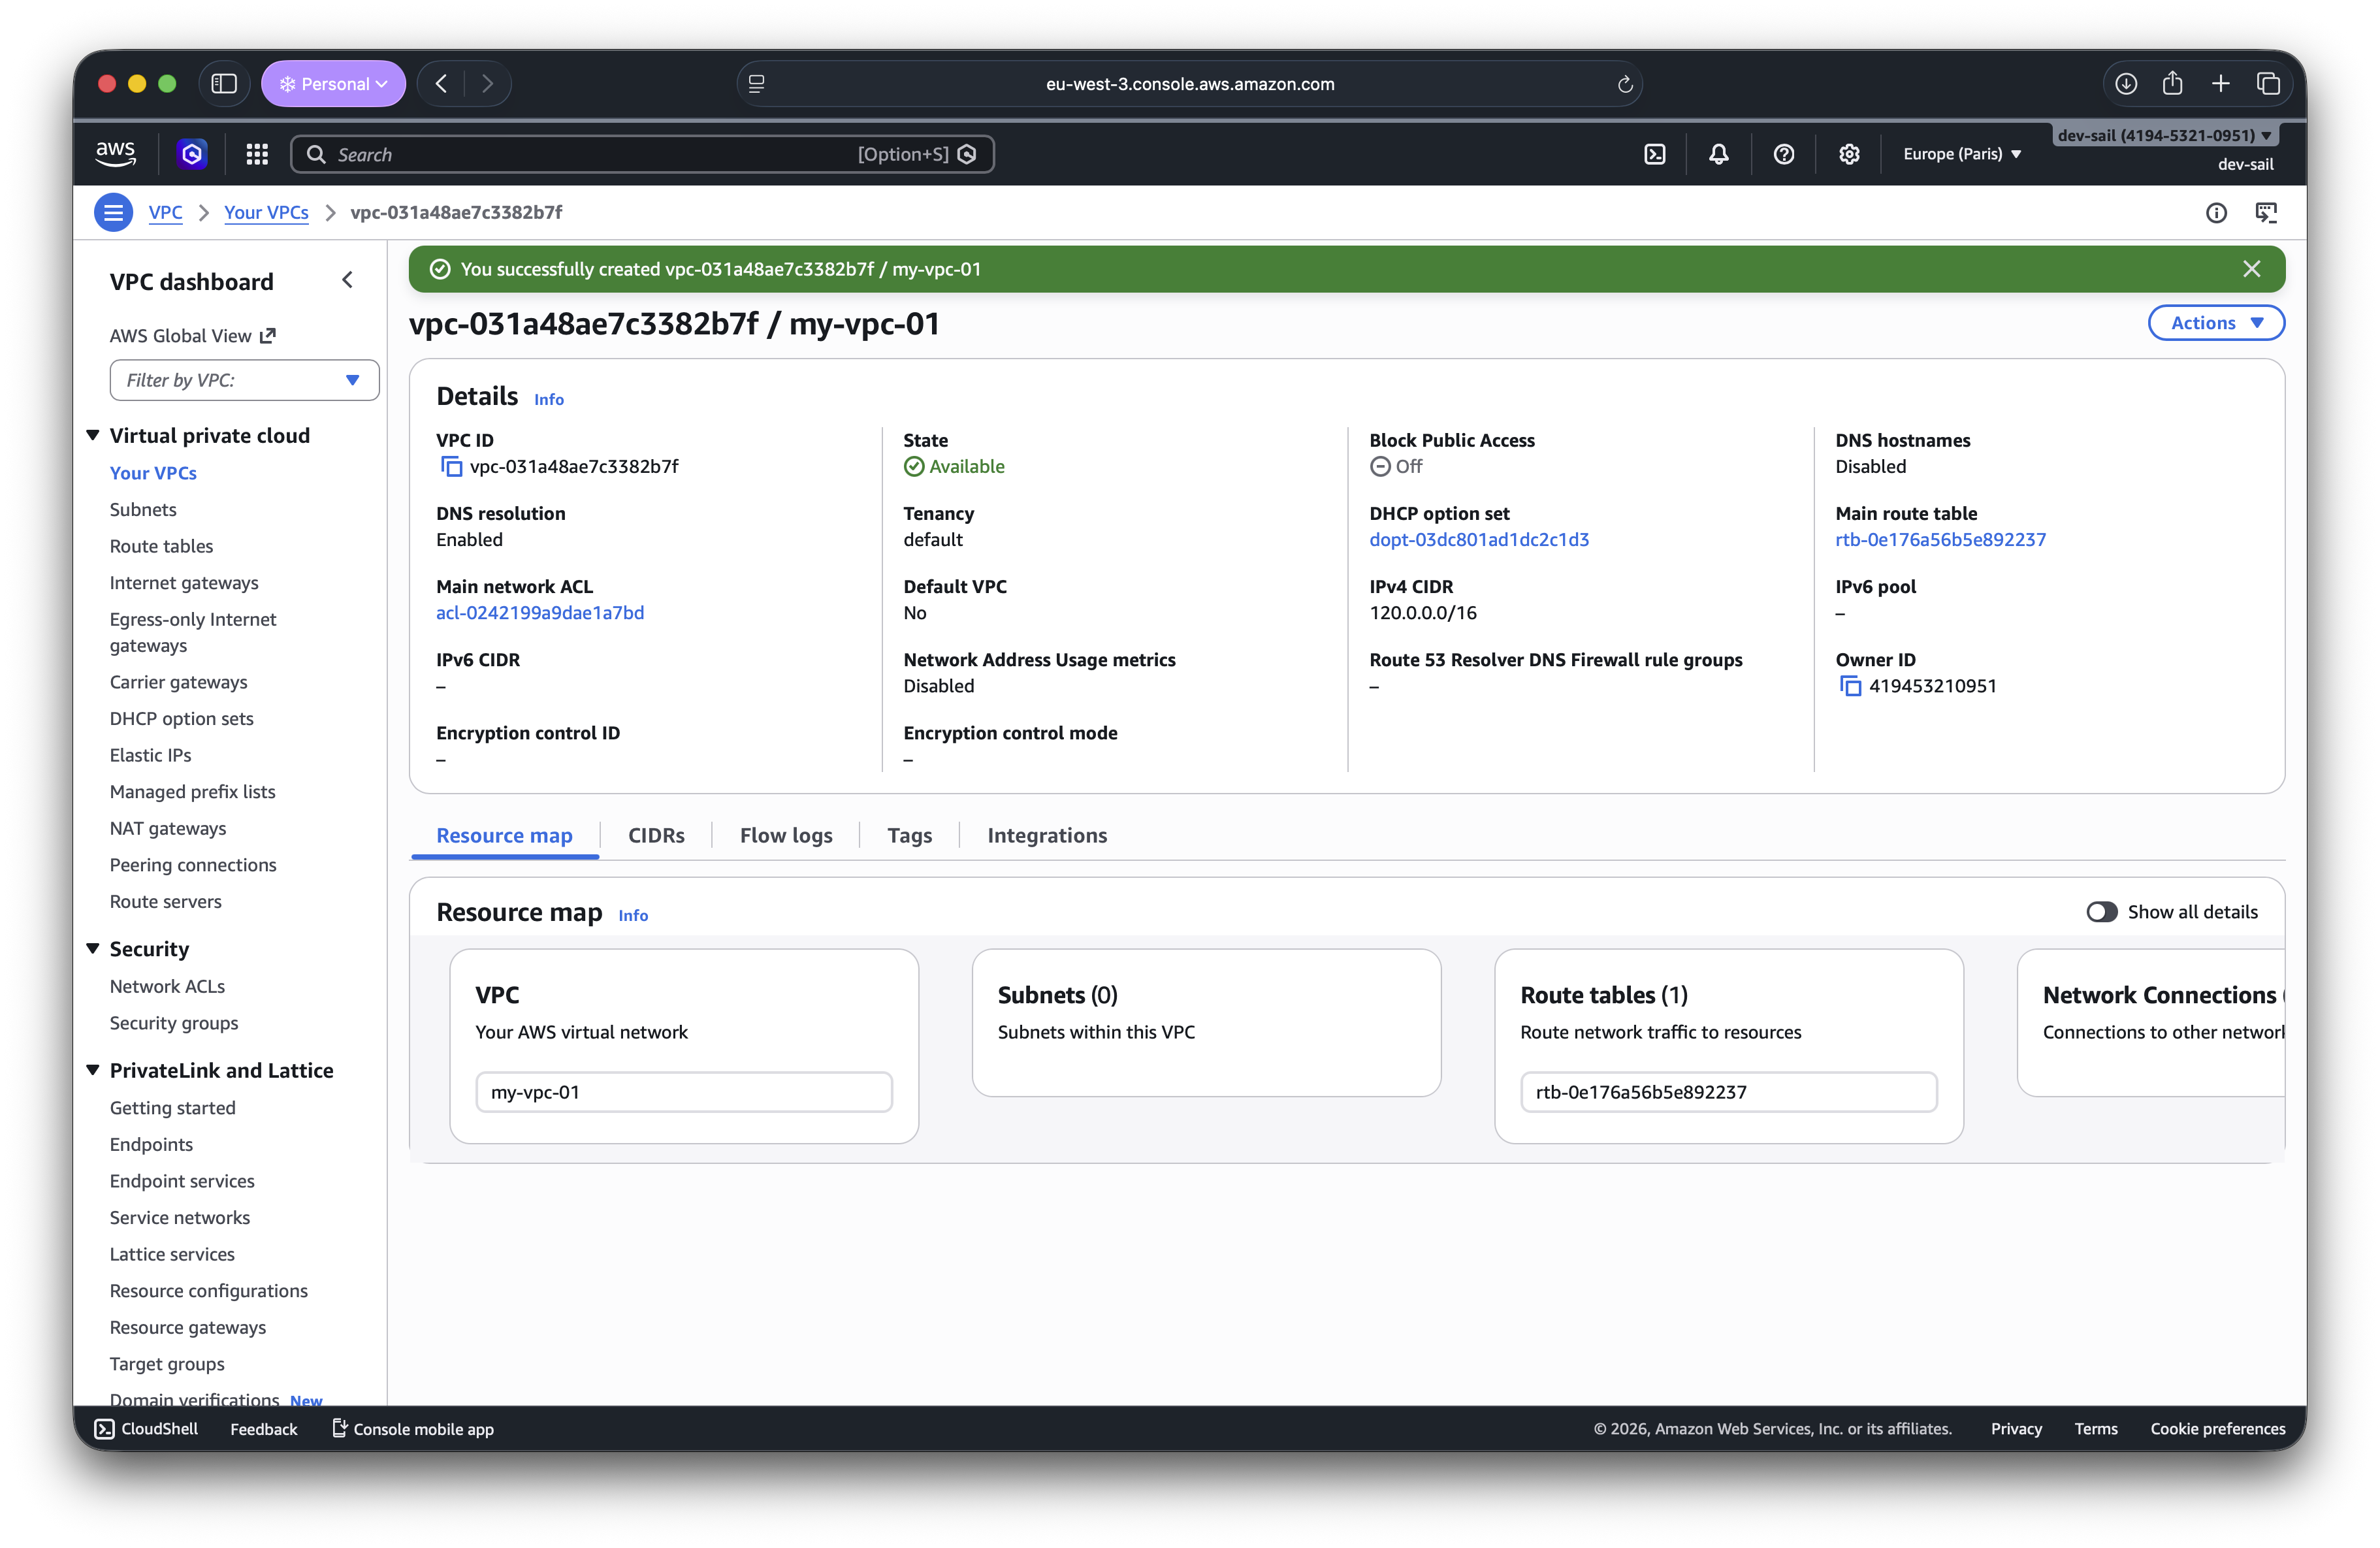
\includegraphics[width=0.75\textwidth]{figures/lab_3/created_vpc.png}
\caption{VPC created successfully}
\end{figure}

%% ============ SECTION 2: Subnet Creation ============ %%
\vspace{8cm}
\section{Subnet Creation}

In VPC service $\rightarrow$ Click on subnets $\rightarrow$ Create subnet

\subsection{Create Public Subnet}

\textbf{Steps:}

\begin{enumerate}
    \item Select the correct VPC
    \item Provide a subnet Name i.e., \texttt{Public}
    \item Assign the IPv4 CIDR block for this subnet \texttt{120.0.3.0/24}
    \item Provide Tags for easy tracking and identification
    \item Click \textbf{Create subnet}
\end{enumerate}

\begin{figure}[H]
\centering
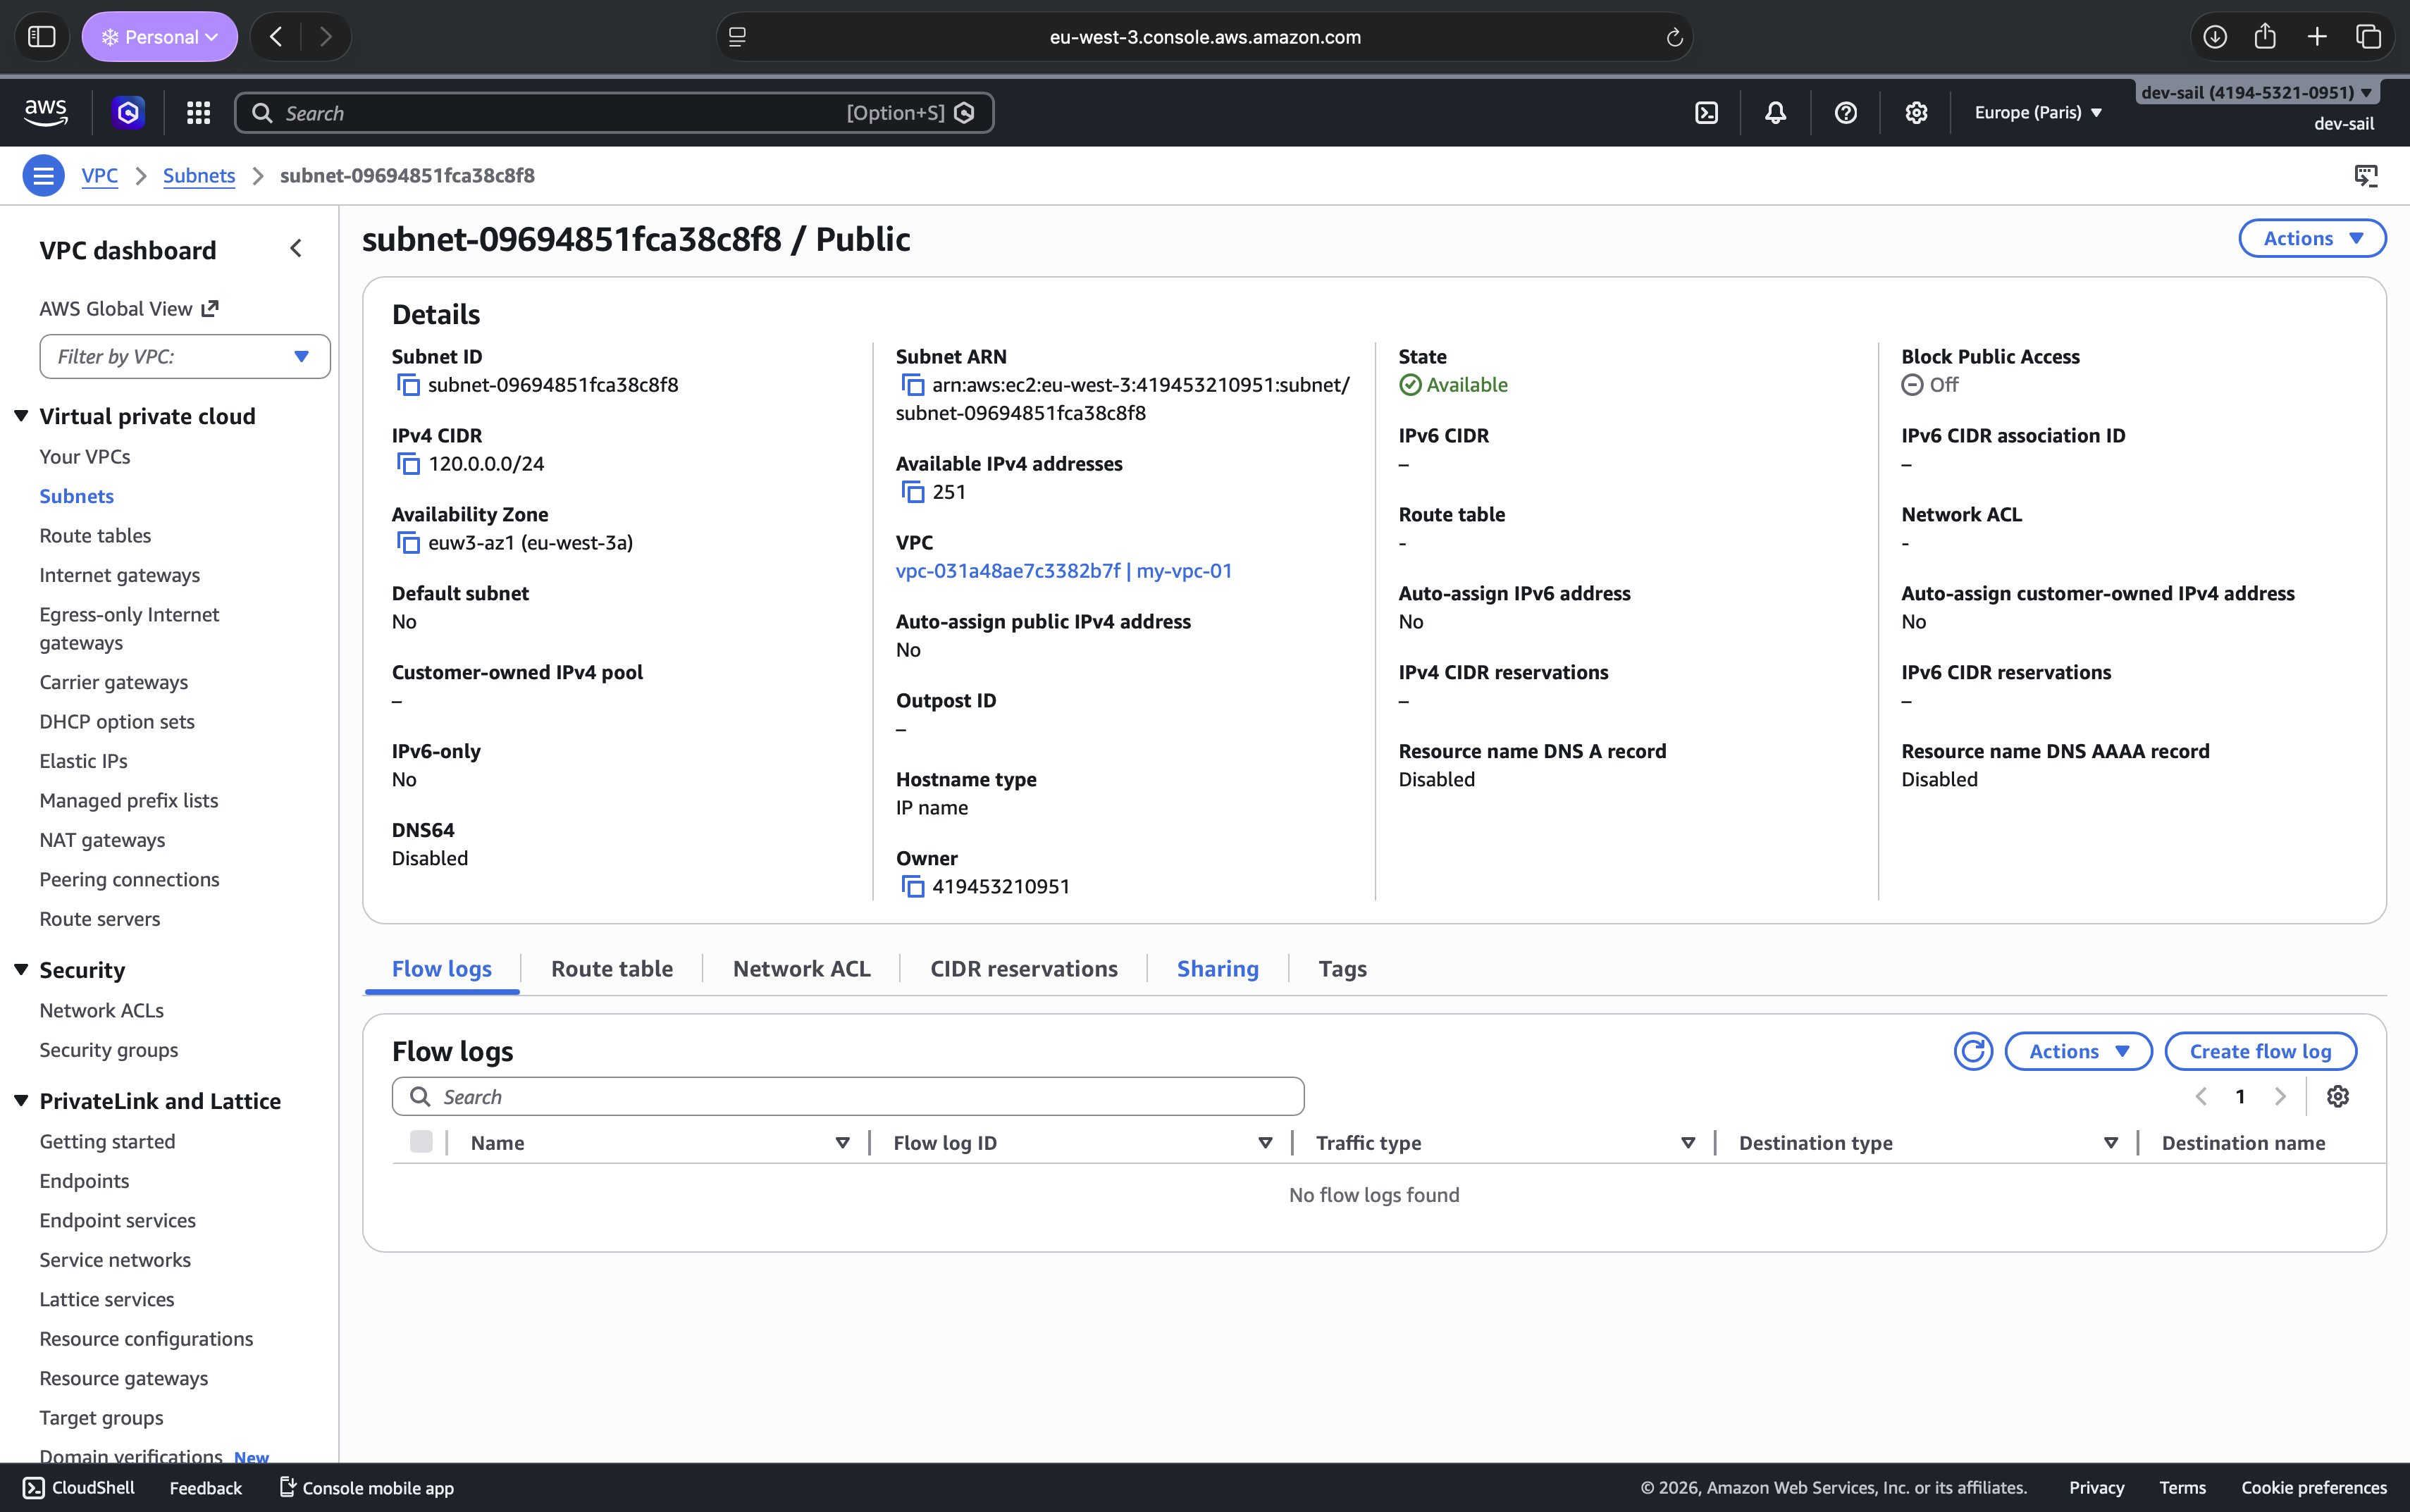
\includegraphics[width=0.75\textwidth]{figures/lab_3/public_subnet.png}
\caption{Public subnet created}
\end{figure}

\subsection{Create Private Subnet 1}

\textbf{Steps:}

\begin{enumerate}
    \item Select the correct VPC
    \item Provide a subnet Name i.e., \texttt{Private1}
    \item Assign the IPv4 CIDR block for this subnet \texttt{120.0.1.0/24}
    \item Provide Tags for easy tracking and identification
    \item Click \textbf{Create subnet}
\end{enumerate}

\begin{figure}[H]
\centering
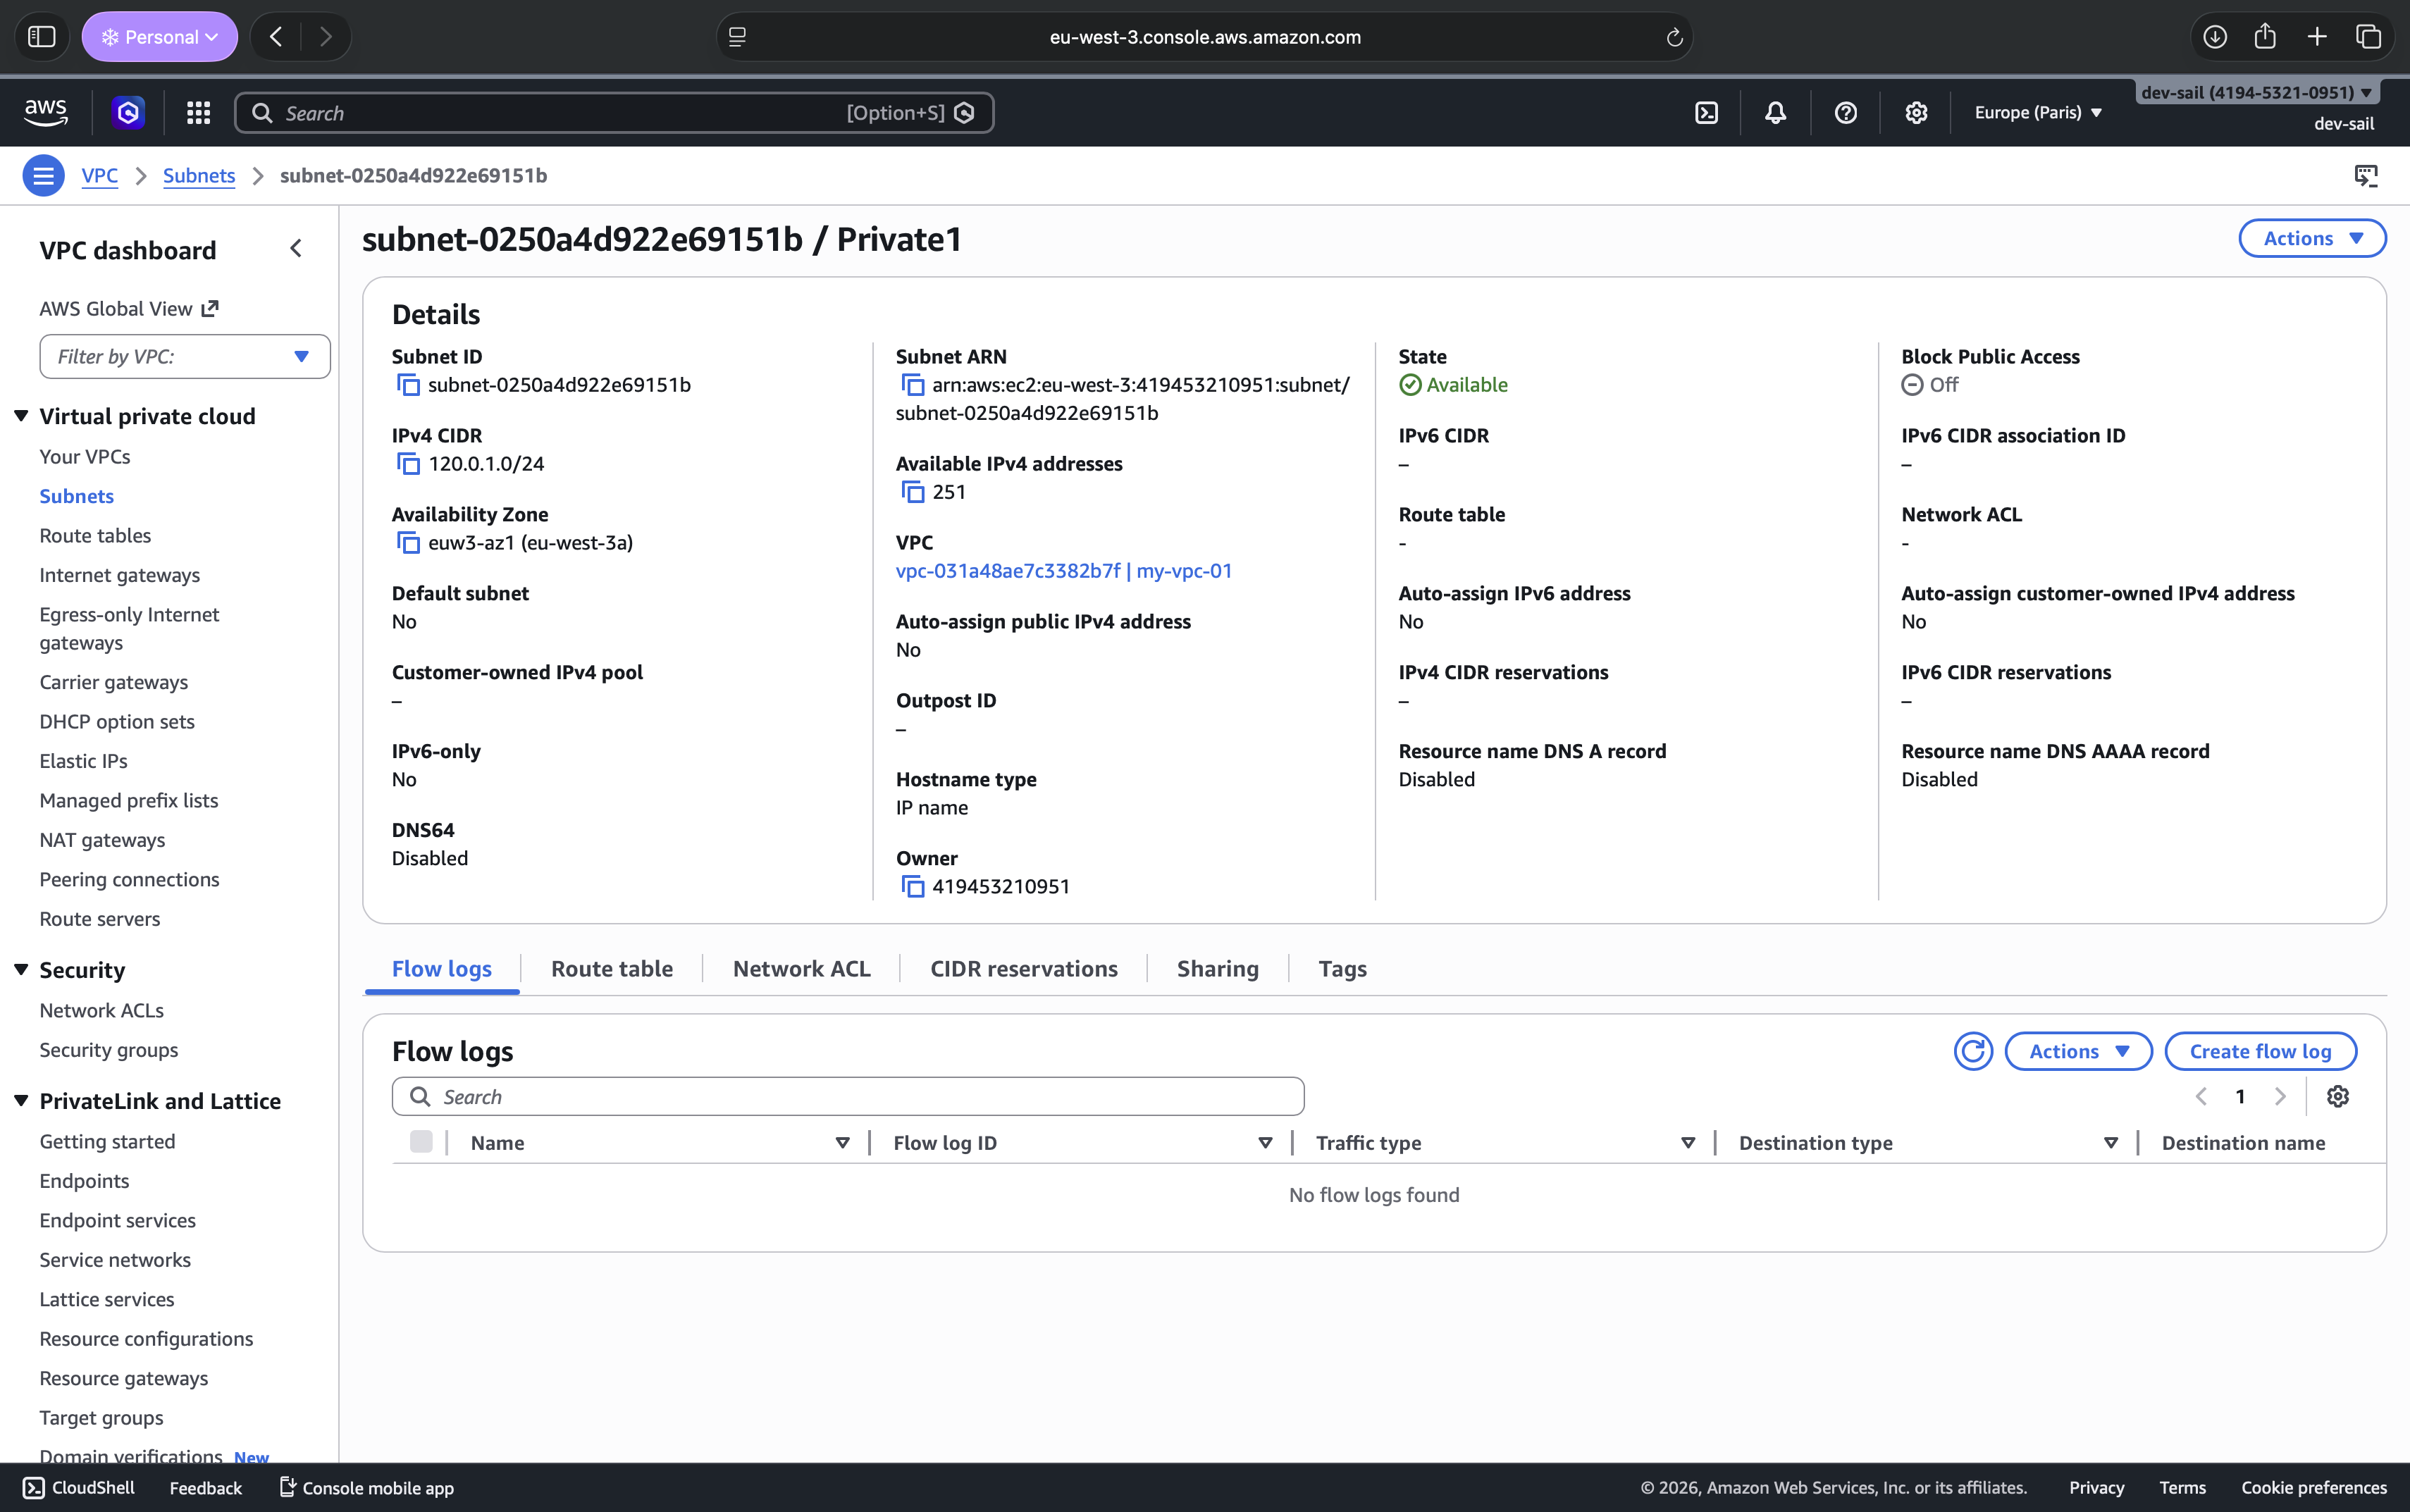
\includegraphics[width=0.75\textwidth]{figures/lab_3/private1_subnet.png}
\caption{Private1 subnet created}
\end{figure}

\vspace{3cm}

\subsection{Create Private Subnet 2}

\textbf{Steps:}

\begin{enumerate}
    \item Select the correct VPC
    \item Provide a subnet Name i.e., \texttt{Private2}
    \item Assign the IPv4 CIDR block for this subnet \texttt{120.0.2.0/24}
    \item Provide Tags for easy tracking and identification
    \item Click \textbf{Create subnet}
\end{enumerate}
\vspace{-0.3cm}
\begin{figure}[H]
\centering
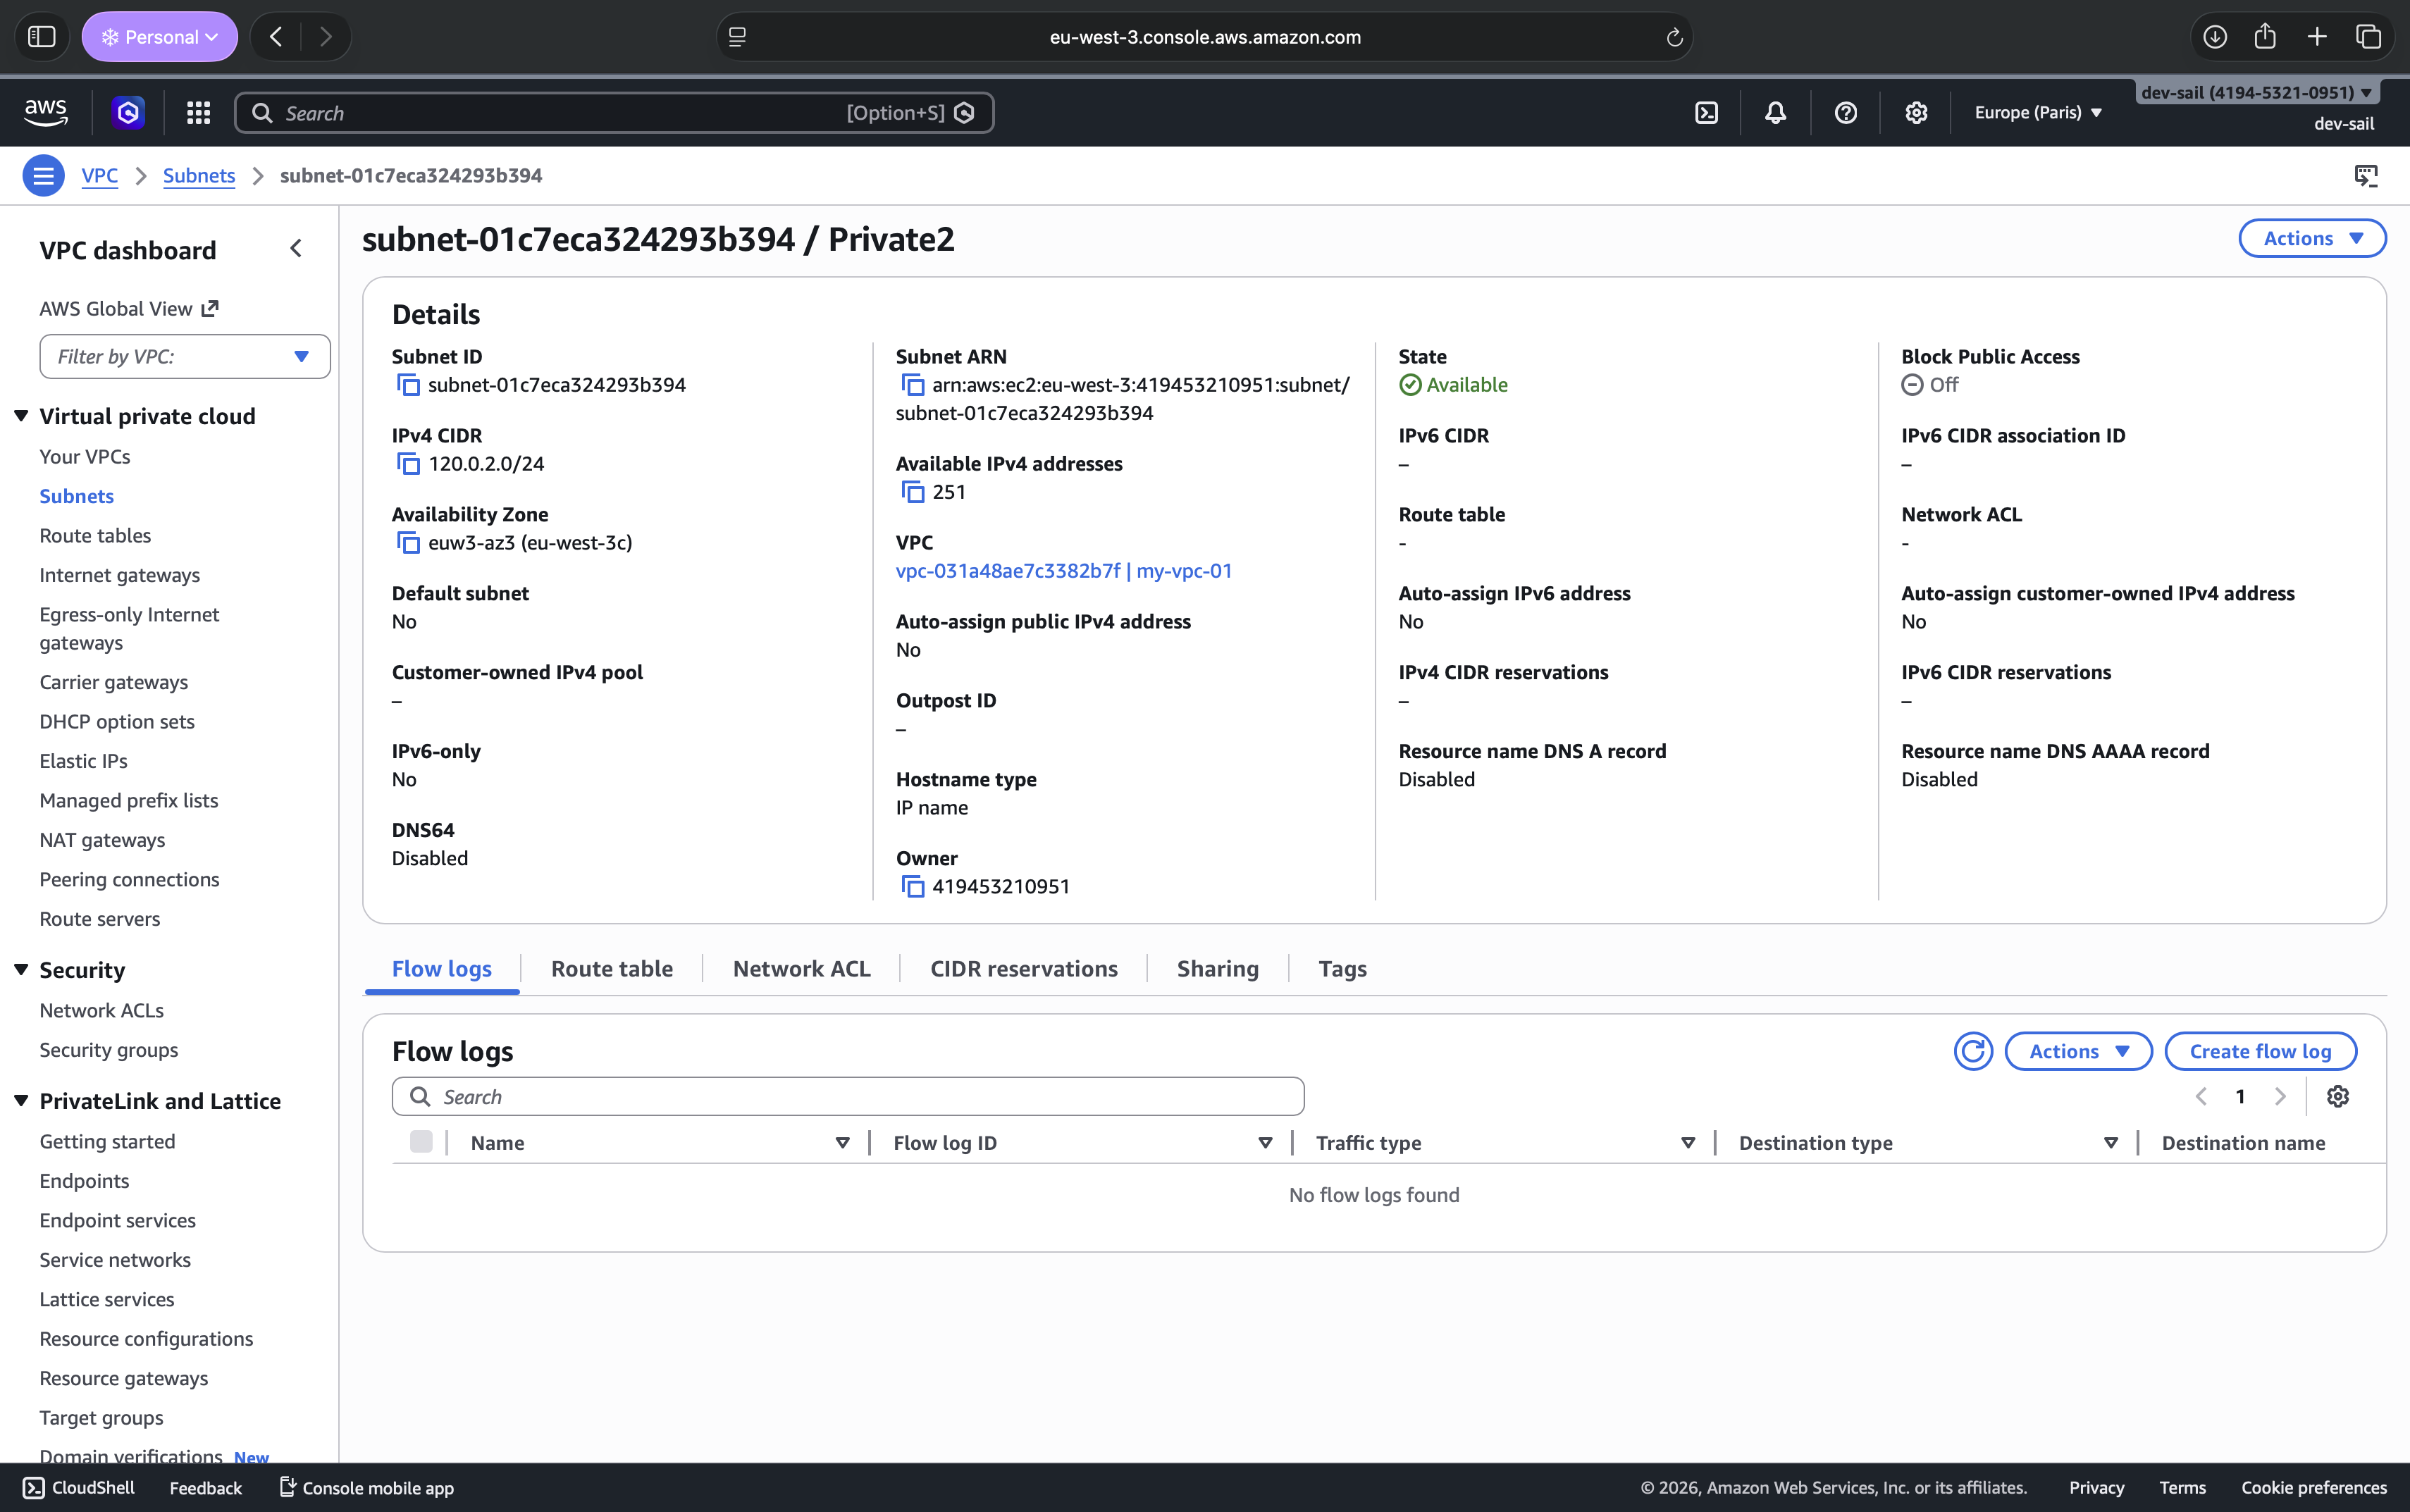
\includegraphics[width=0.75\textwidth]{figures/lab_3/private2_subnet.png}
\caption{Private2 subnet created}
\end{figure}

\vspace{11cm}

%% ============ SECTION 3: Internet Gateway ============ %%
\section{Internet Gateway}

In VPC service $\rightarrow$ Internet gateways $\rightarrow$ Create internet gateway

\subsection{Create Internet Gateway}

\textbf{Steps:}

\begin{enumerate}
    \item Provide name: \texttt{igw1}
    \item Click \textbf{Create internet gateway}
    \item Select the created gateway and click \textbf{Actions} $\rightarrow$ \textbf{Attach to VPC}
    \item Select \textbf{MyVPC1}
    \item Click \textbf{Attach internet gateway}
\end{enumerate}

\begin{figure}[H]
\centering
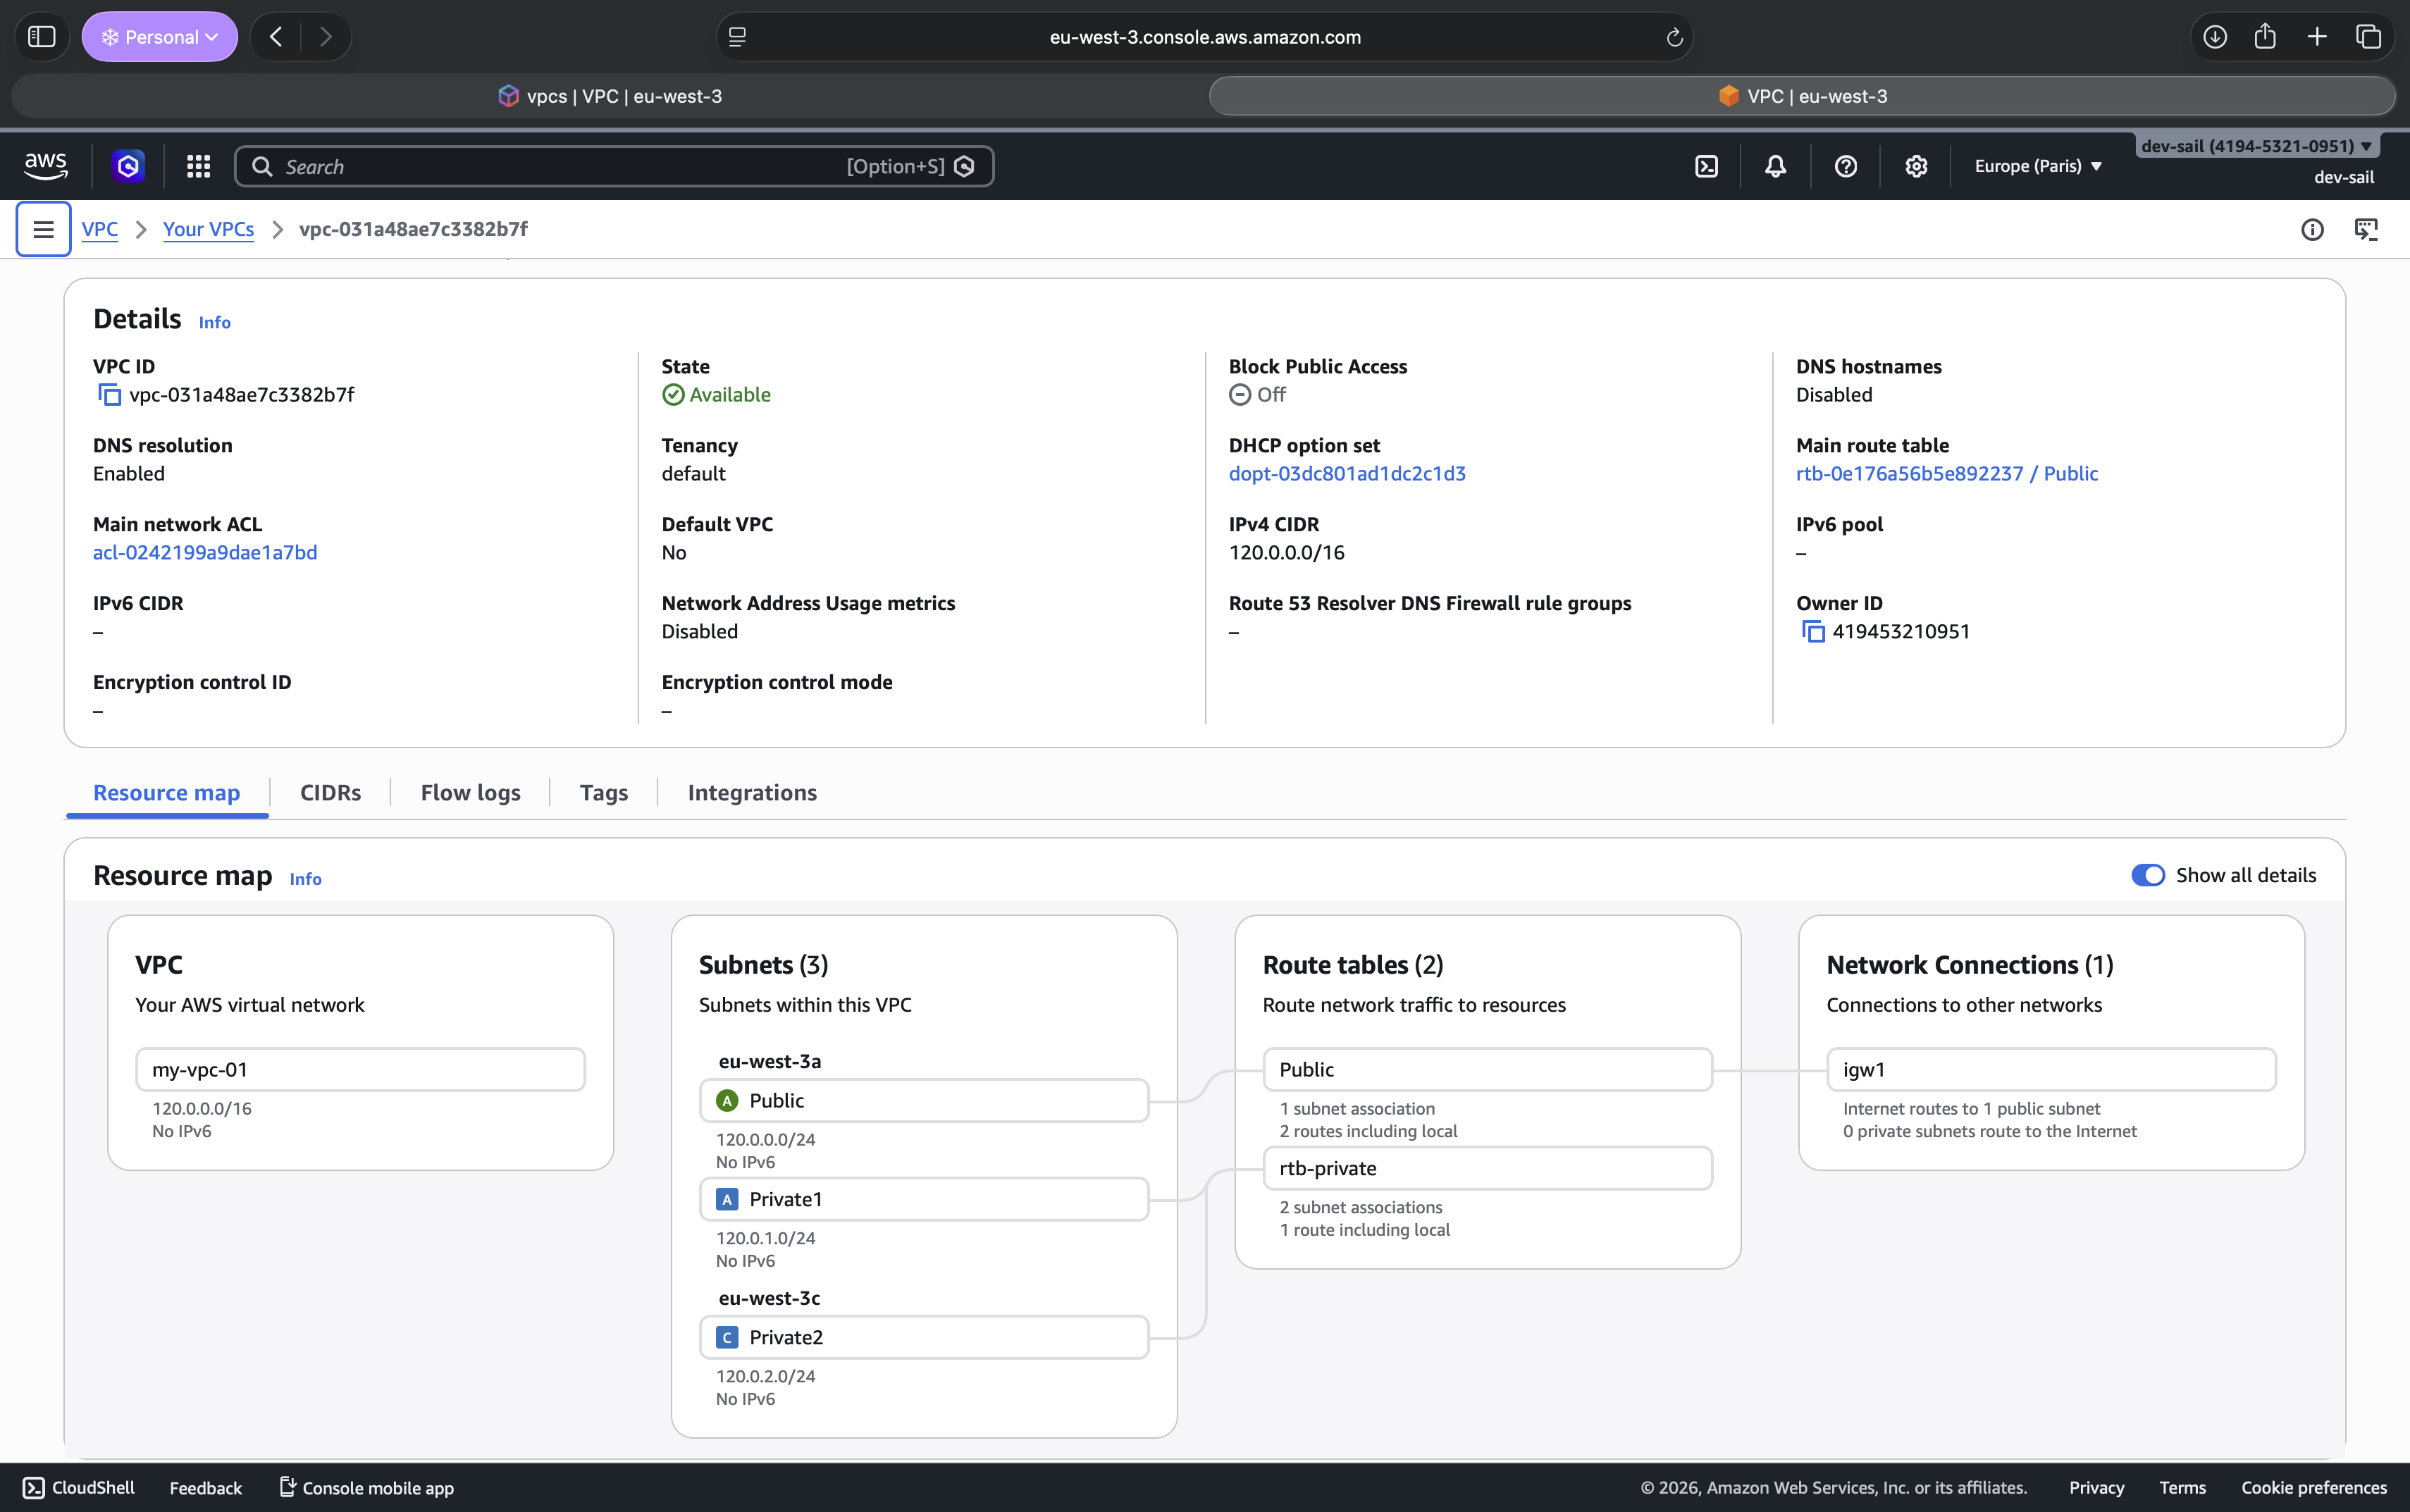
\includegraphics[width=0.75\textwidth]{figures/lab_3/vpc_resource_map.png}
\caption{VPC Resource Map}
\end{figure}

%% ============ SECTION 4: Route Tables ============ %%
\vspace{9cm}
\section{Route Tables}

In VPC service $\rightarrow$ Route tables

\subsection{Public Route Table}

\textbf{Steps:}

\begin{enumerate}
    \item Navigate to Route tables
    \item Edit the public route table and add the following route:
    \begin{itemize}
        \item \textbf{Destination:} 0.0.0.0/0
        \item \textbf{Target:} Internet Gateway (igw1)
    \end{itemize}
\end{enumerate}

\begin{figure}[H]
\centering
\begin{minipage}{0.48\textwidth}
    \centering
    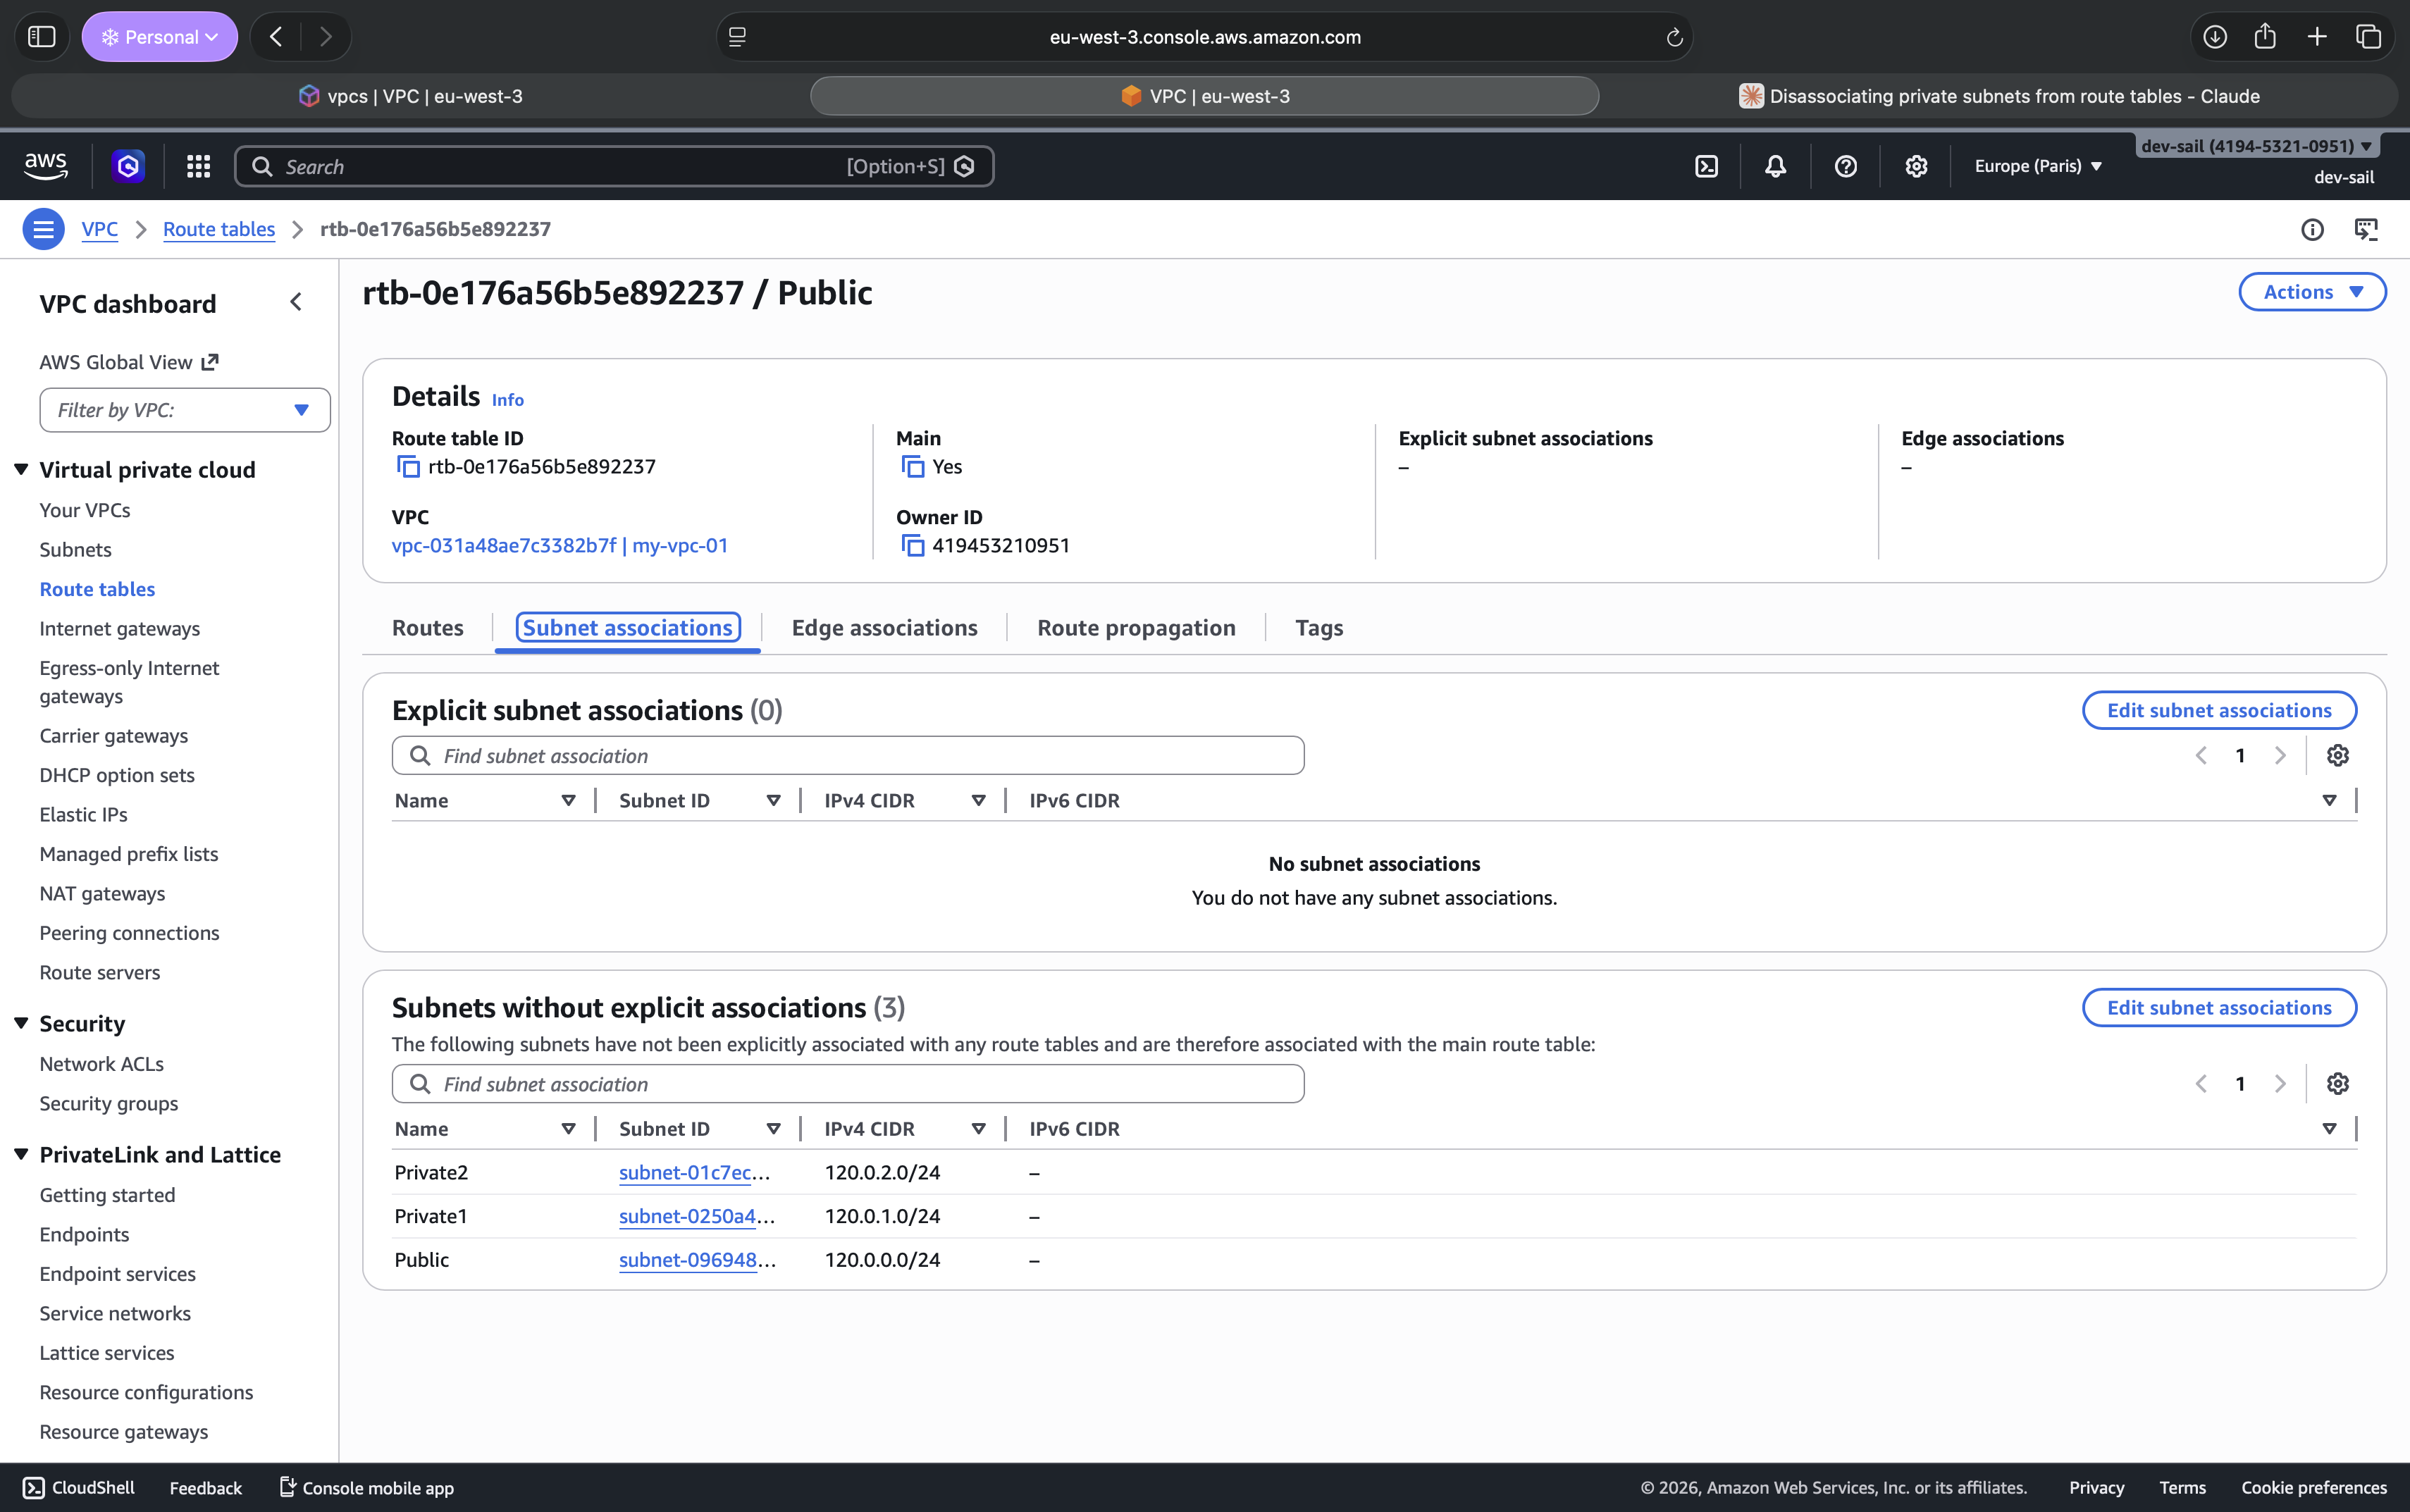
\includegraphics[width=\linewidth]{figures/lab_3/public_route_table_before.png}
    \captionof{figure}{Public route table before}
\end{minipage}\hfill
\begin{minipage}{0.48\textwidth}
    \centering
    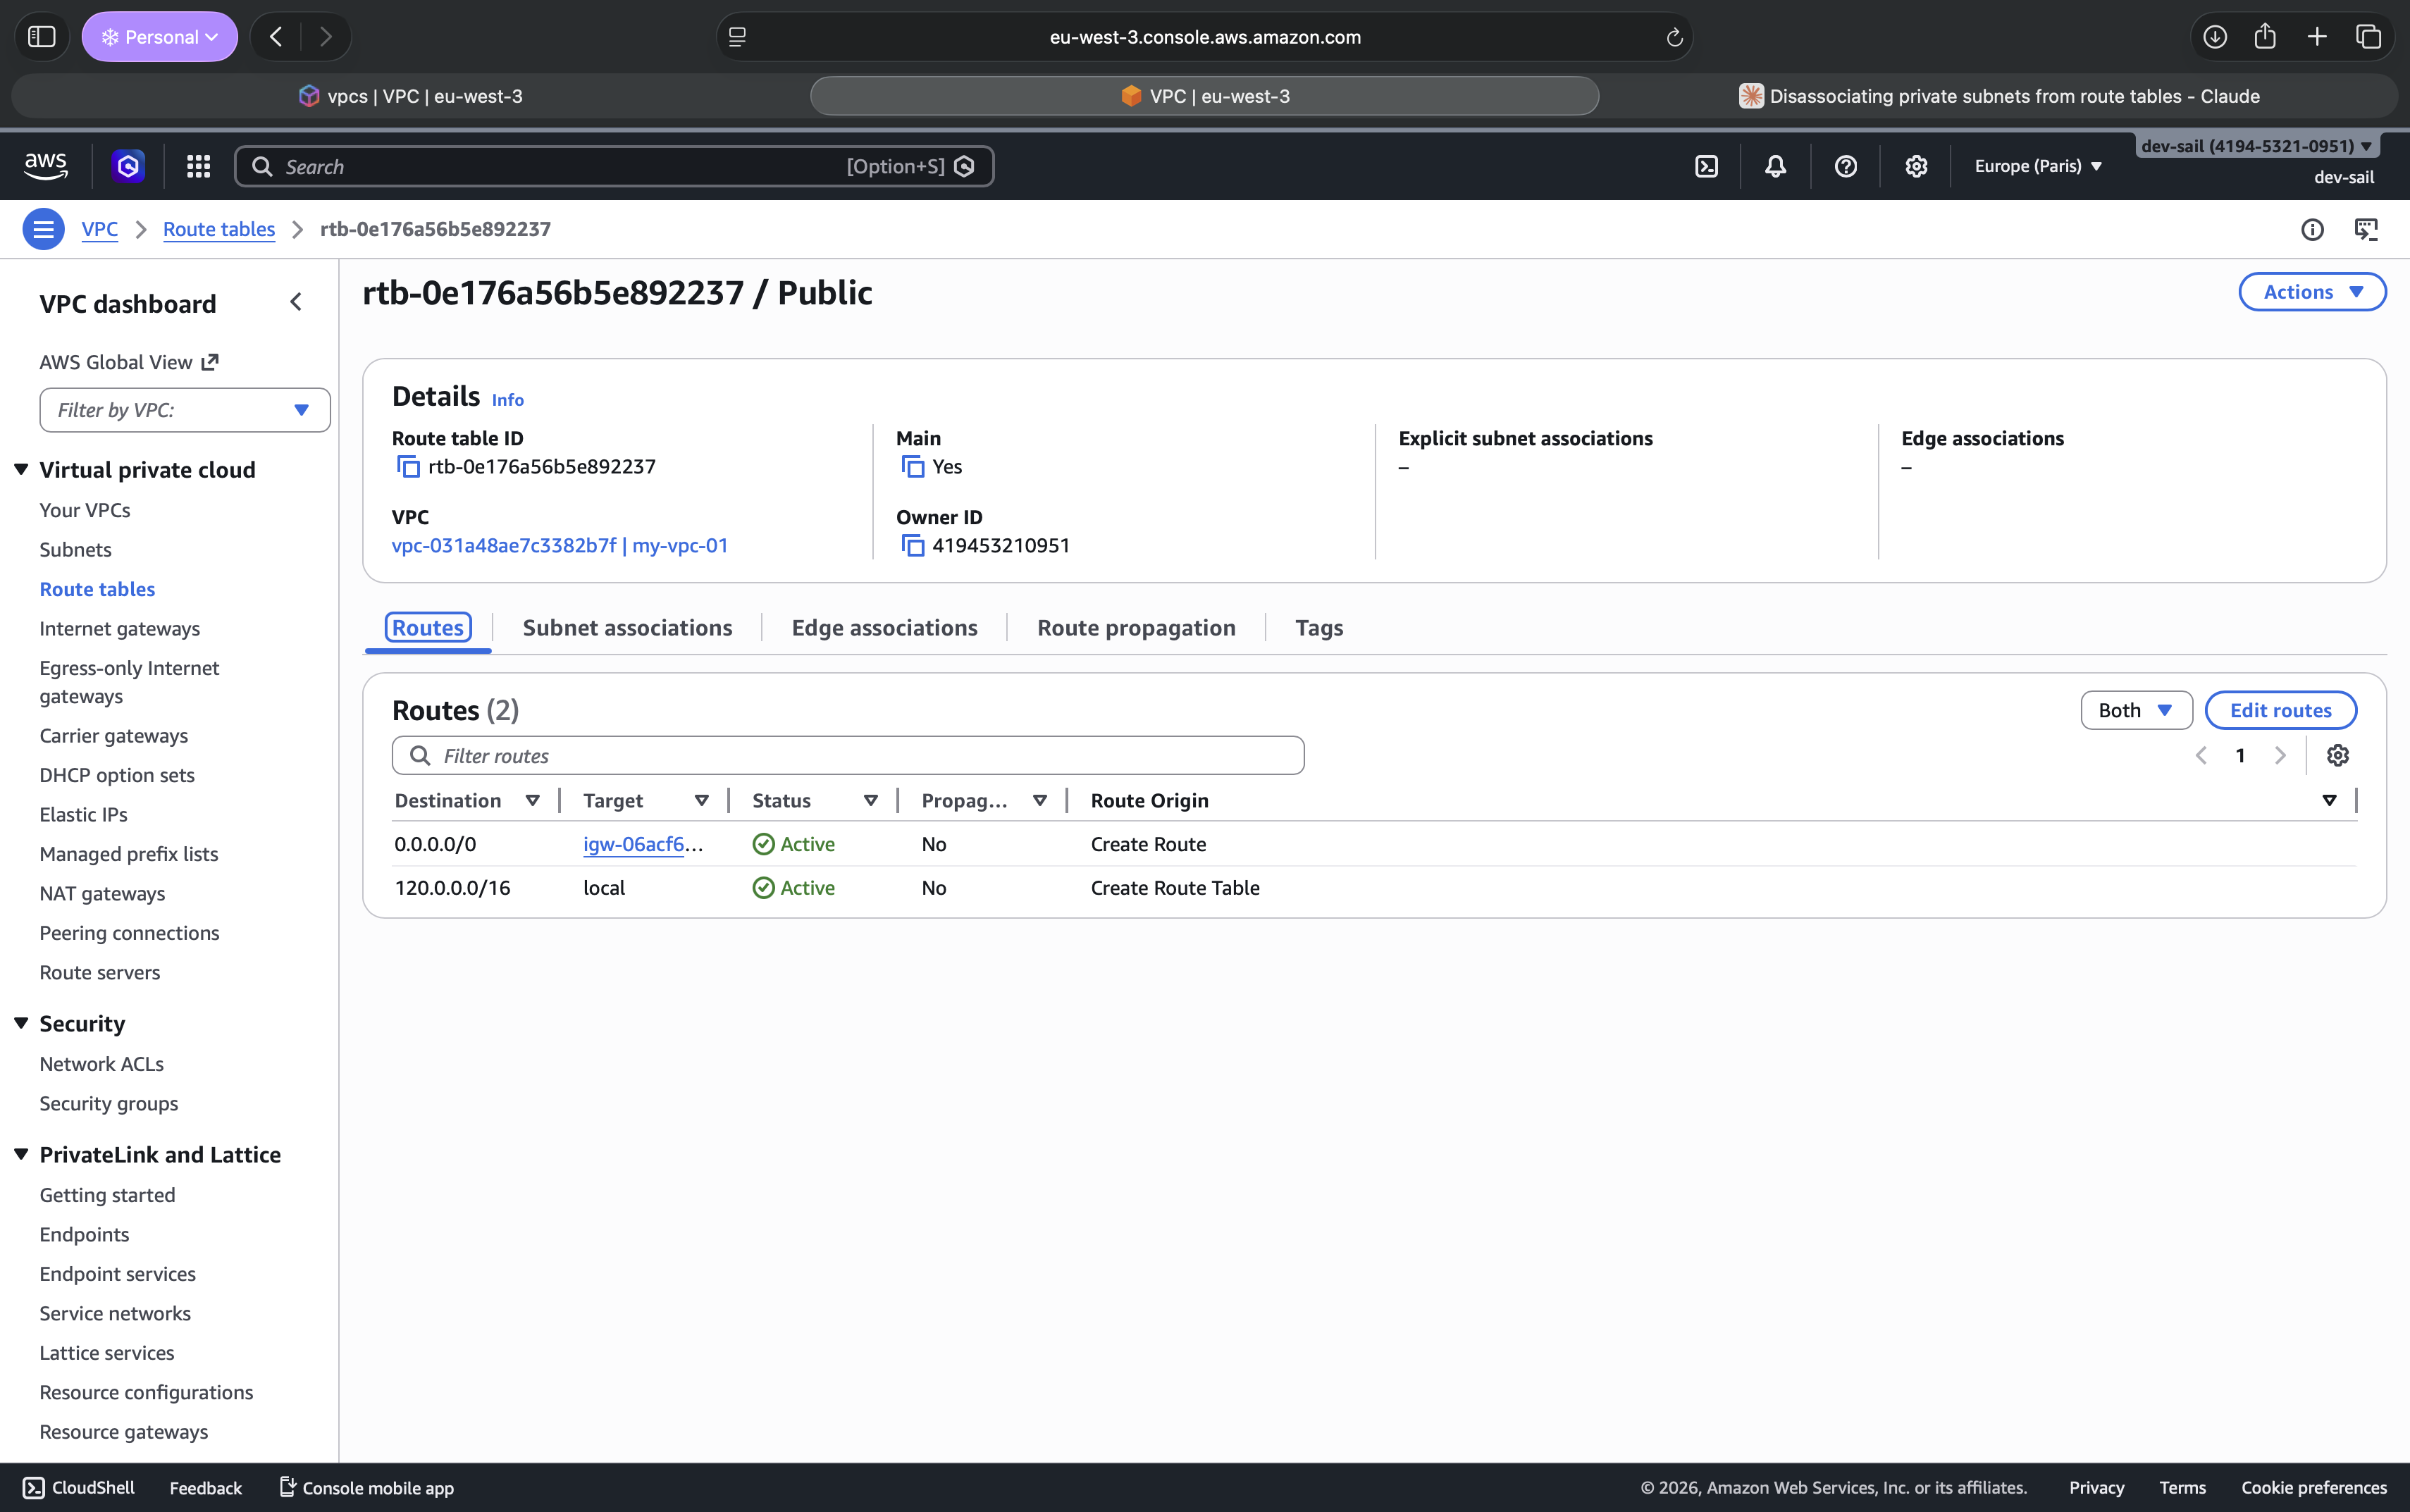
\includegraphics[width=\linewidth]{figures/lab_3/public_route_table_with_igw.png}
    \captionof{figure}{Adding IGW route}
\end{minipage}
\end{figure}

\begin{figure}[H]
\centering
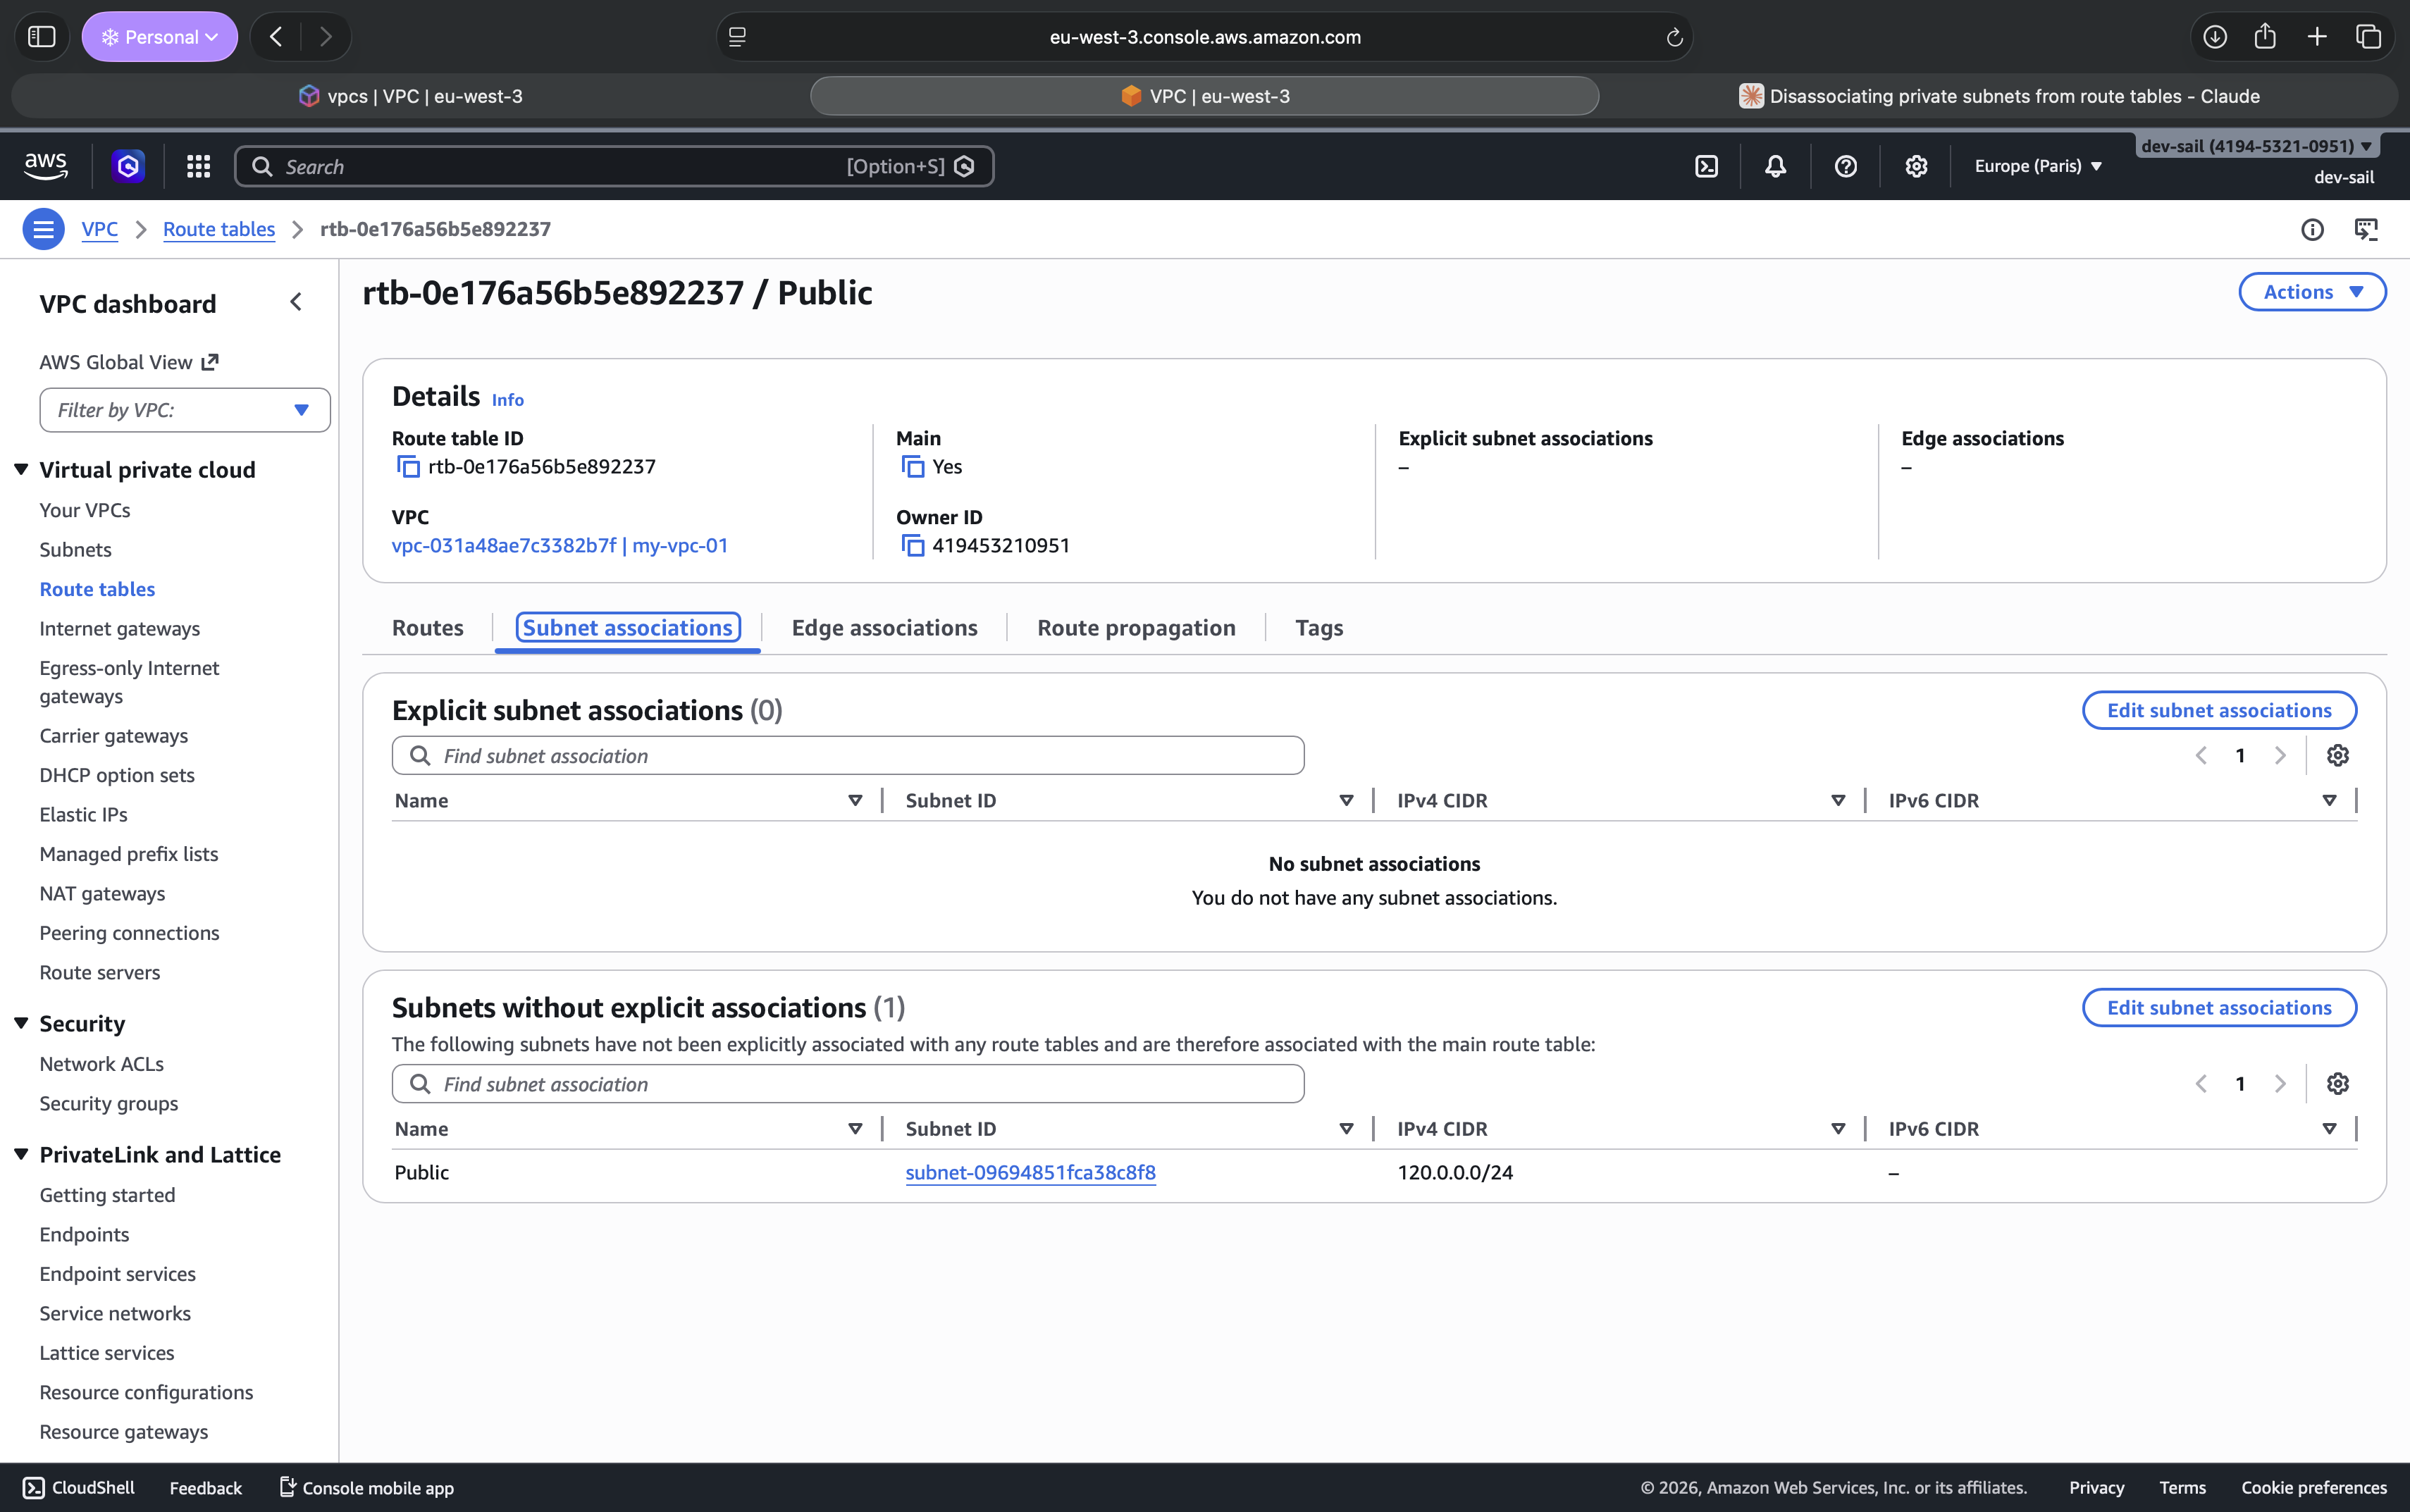
\includegraphics[width=0.75\textwidth]{figures/lab_3/public_route_table_after.png}
\caption{Public route table after adding IGW}
\end{figure}

\subsection{Private Route Table}

\textbf{Steps:}

\begin{enumerate}
    \item Navigate to Route tables
    \item Click \textbf{Create route table}
    \item Provide name: \texttt{rtb-private}
    \item Select the VPC (\textbf{MyVPC1})
    \item Click \textbf{Create route table}
    \item Associate the private subnets (Private1 and Private2) with this route table
\end{enumerate}

\begin{figure}[H]
\centering
\begin{minipage}{0.48\textwidth}
    \centering
    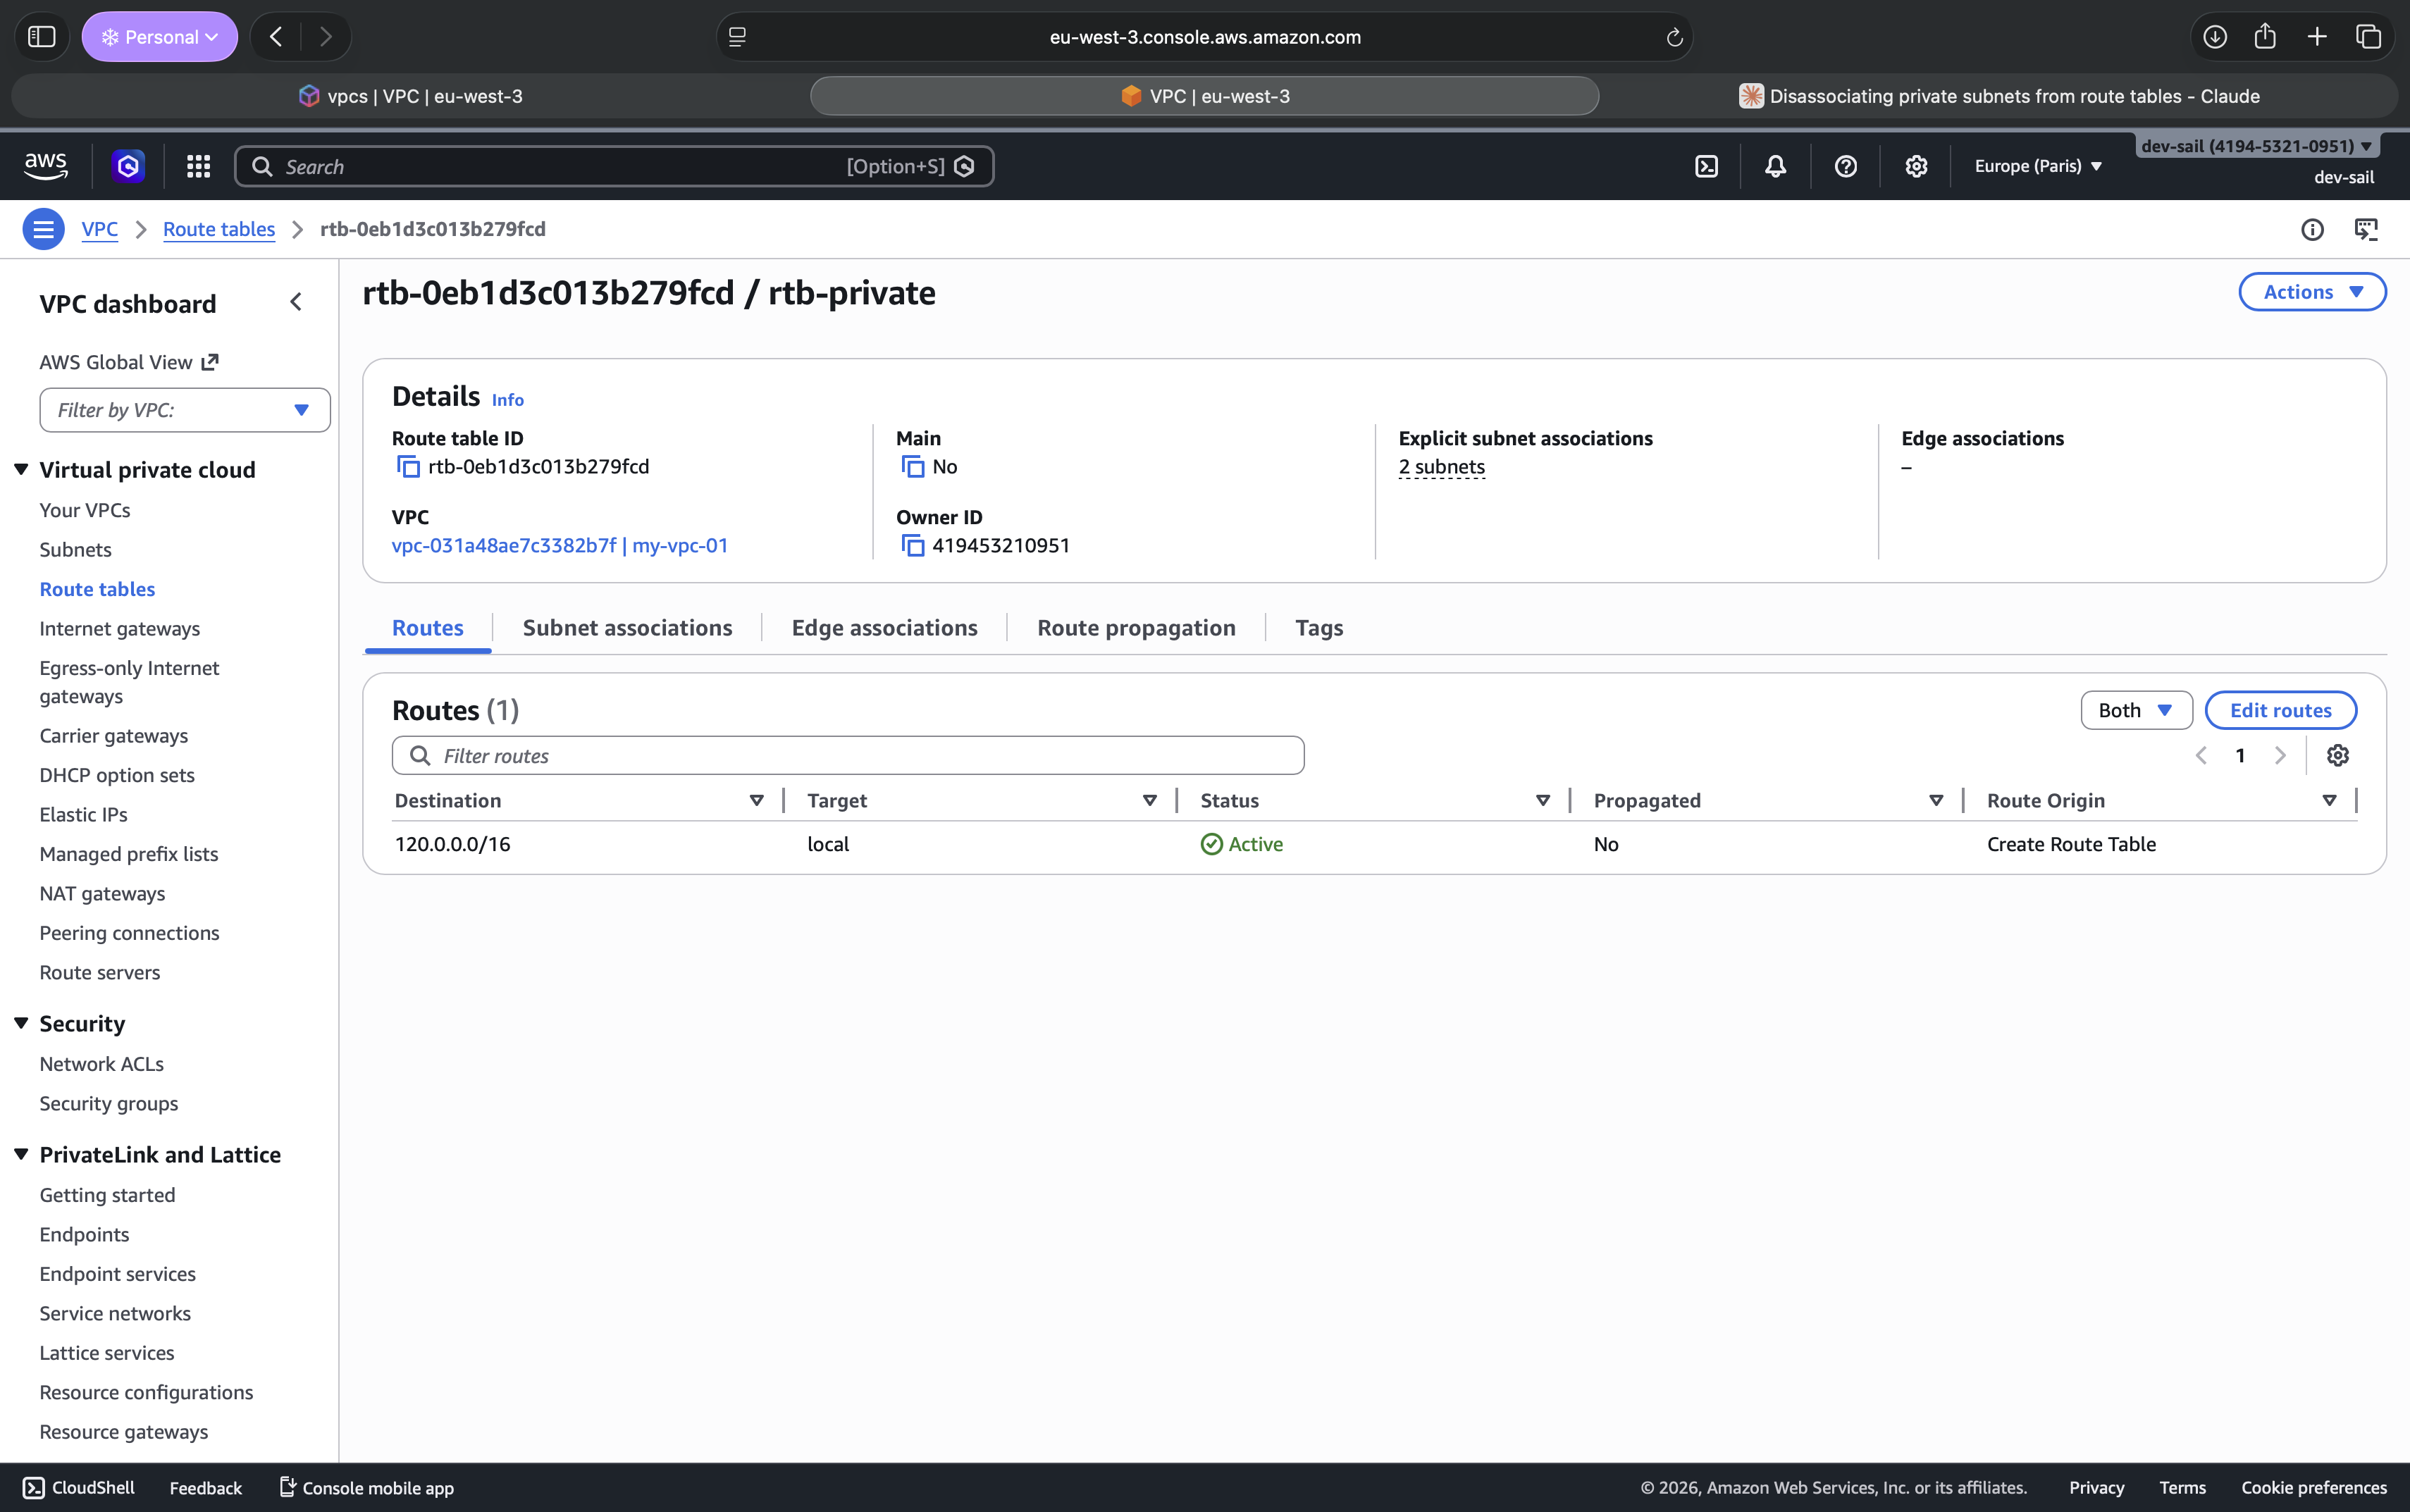
\includegraphics[width=\linewidth]{figures/lab_3/private_route_table_routes.png}
    \captionof{figure}{Private route table routes}
\end{minipage}\hfill
\begin{minipage}{0.48\textwidth}
    \centering
    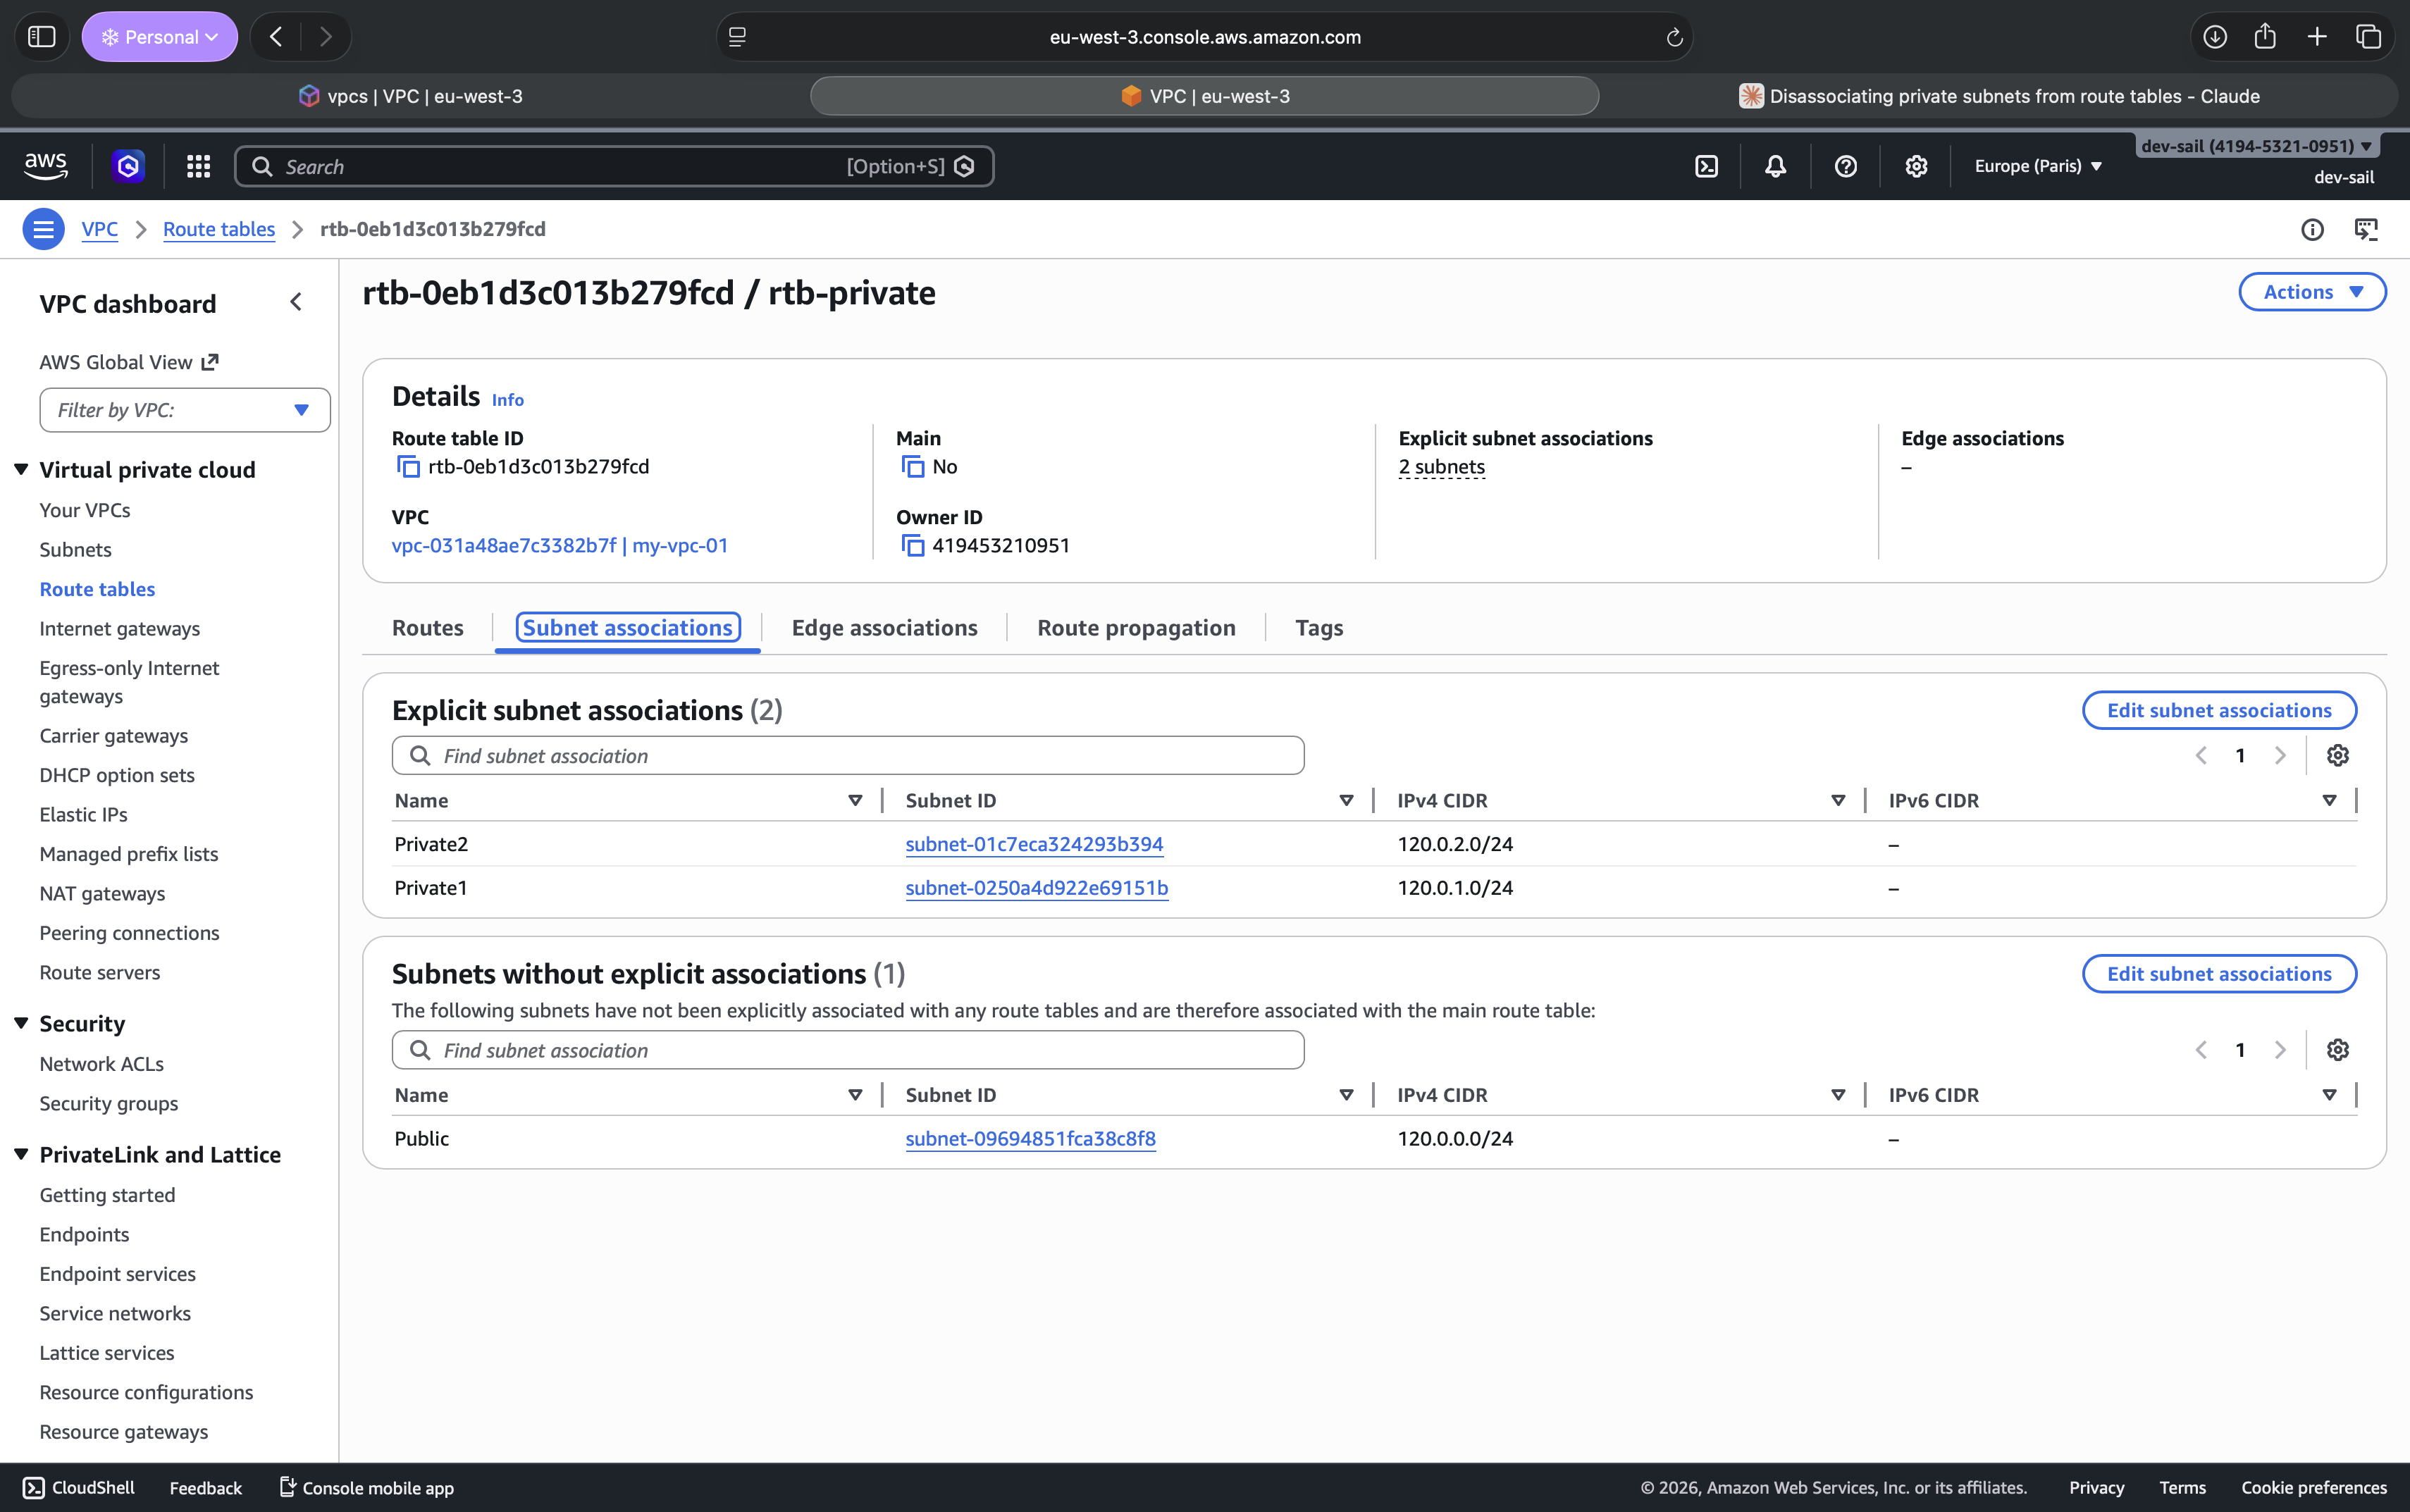
\includegraphics[width=\linewidth]{figures/lab_3/private_route_table_subnets.png}
    \captionof{figure}{Private subnets association}
\end{minipage}
\end{figure}

%% ============ SECTION 5: NAT Gateway ============ %%
\section{NAT Gateway}

In VPC service $\rightarrow$ NAT gateways $\rightarrow$ Create NAT gateway

\subsection{Create NAT Gateway}

\textbf{Steps:}

\begin{enumerate}
    \item Provide name: \texttt{my-nat-gateway1}
    \item Select Subnet: Public subnet
    \item Select Connectivity Type: Public
    \item Click \textbf{Allocate Elastic IP}
    \item Click \textbf{Create NAT gateway}
\end{enumerate}

\begin{figure}[H]
\centering
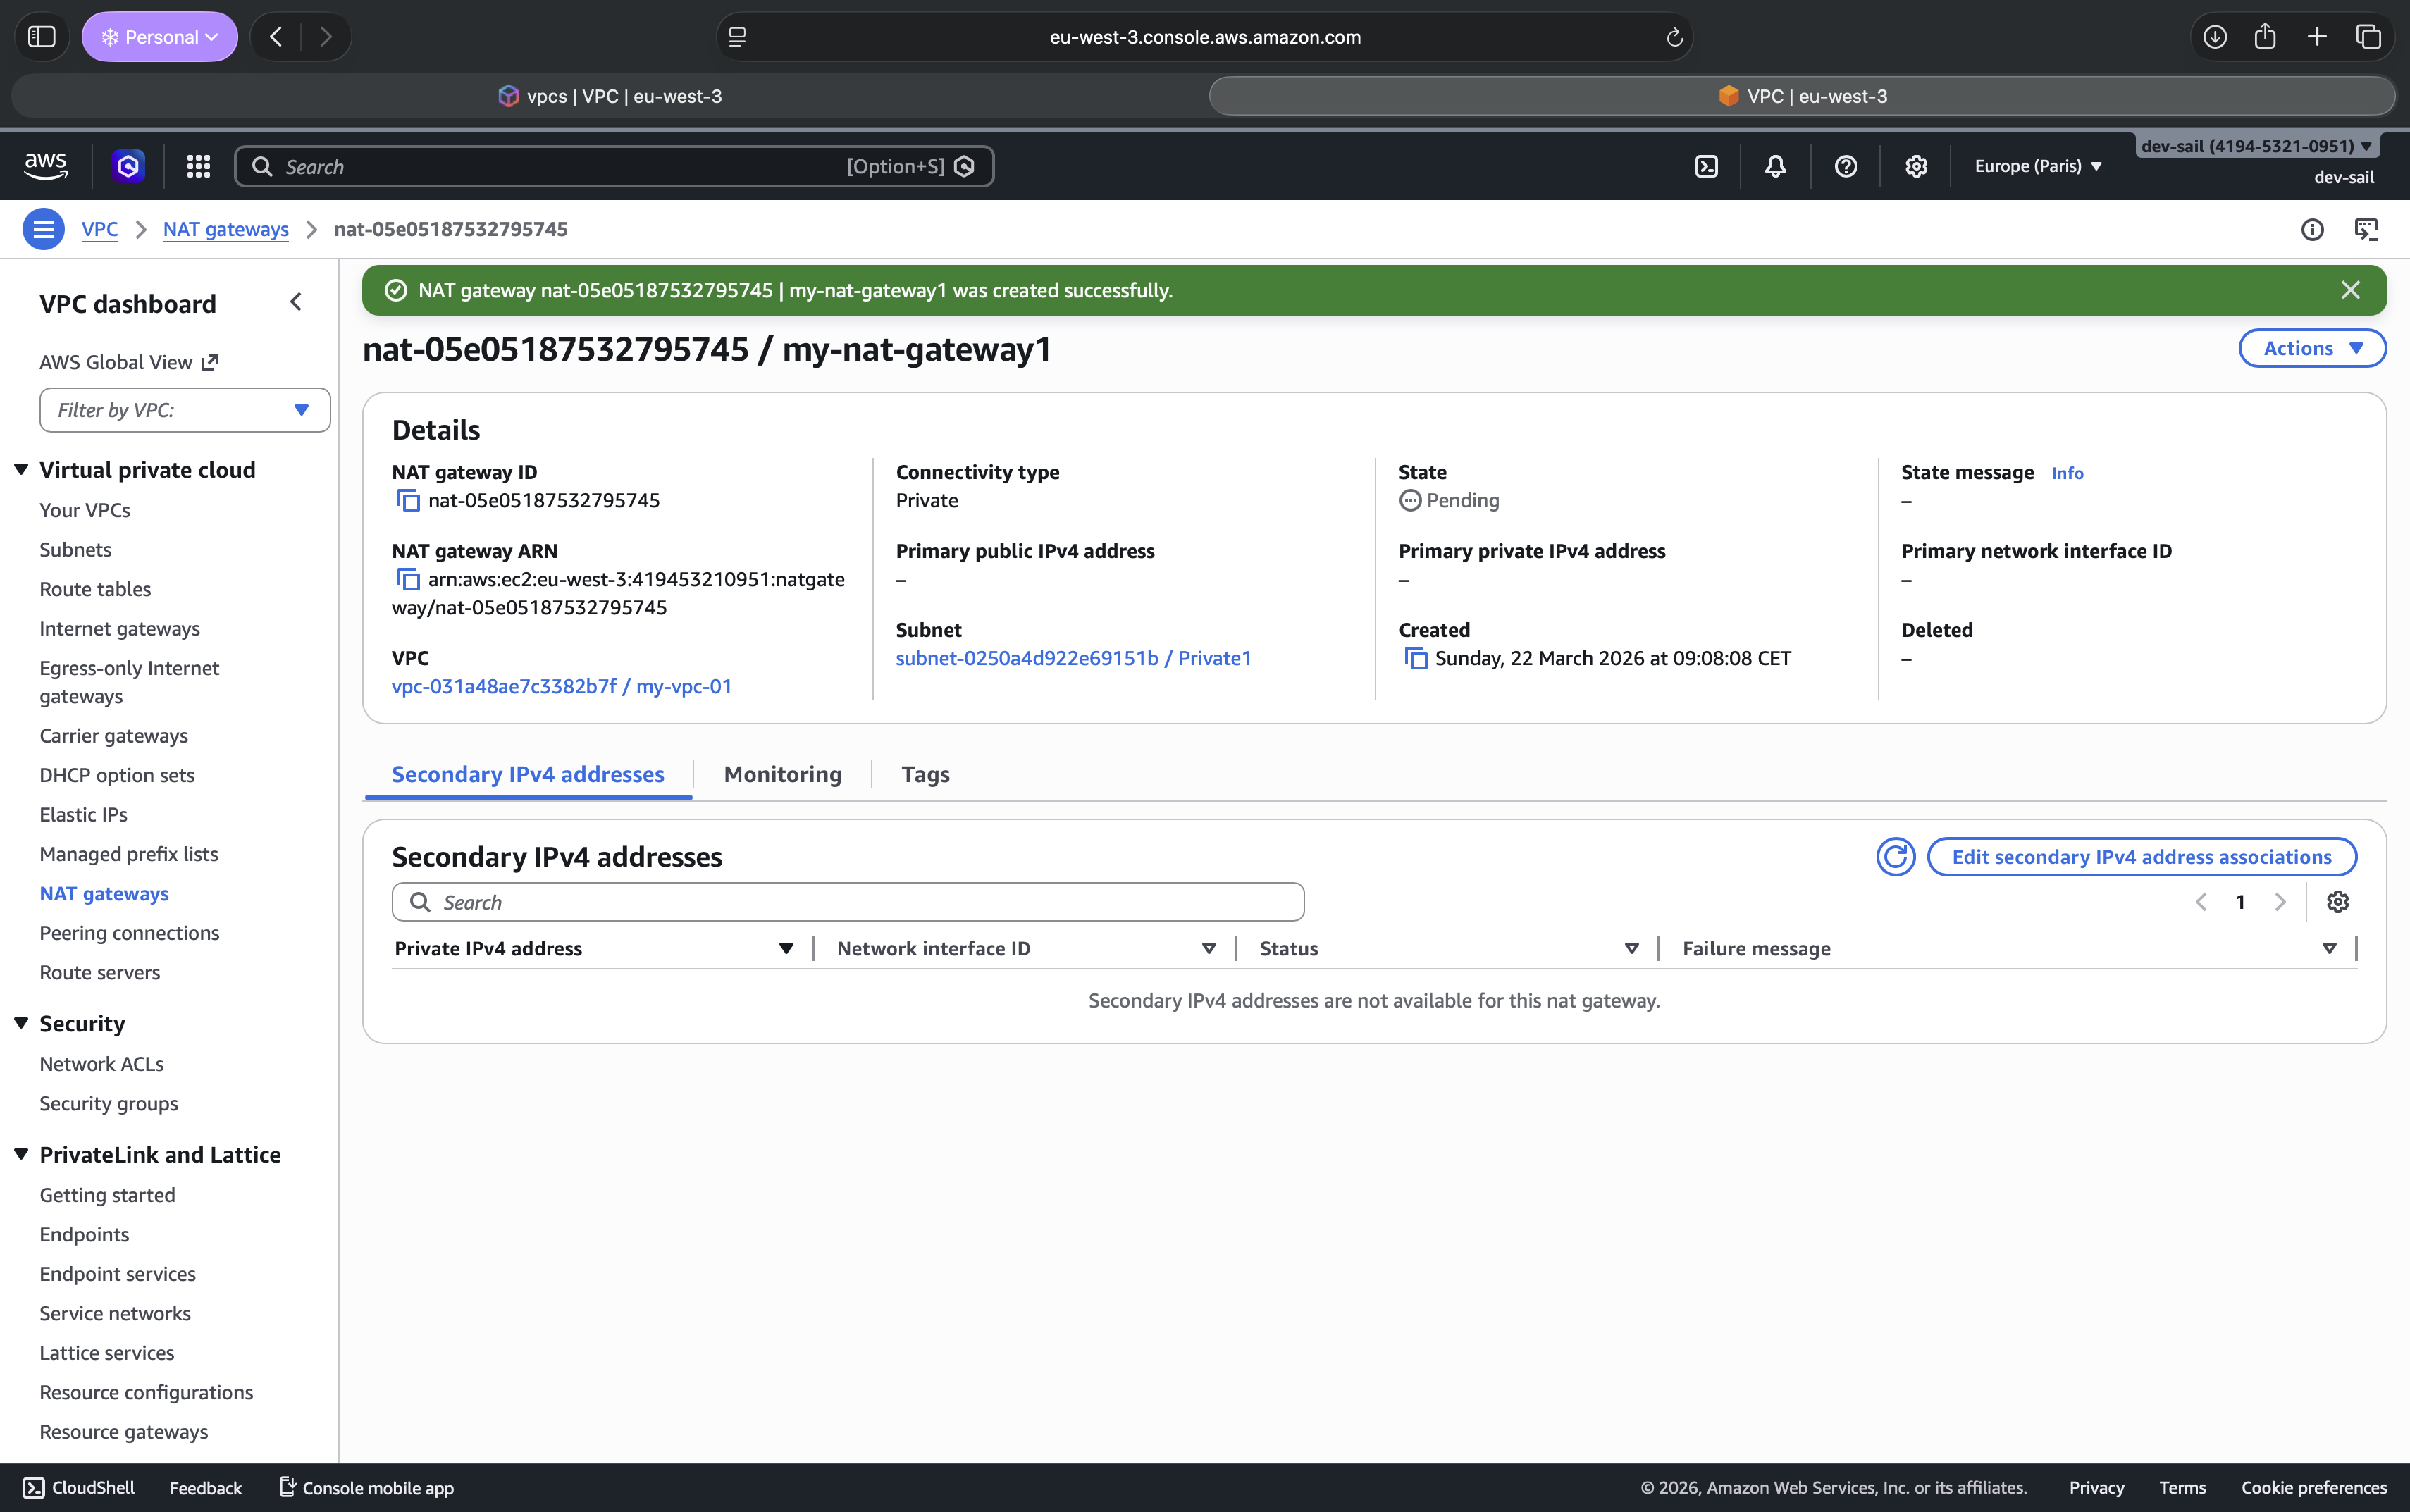
\includegraphics[width=0.75\textwidth]{figures/lab_3/nat_gateway.png}
\caption{NAT Gateway created}
\end{figure}

\subsection{Configure Private Route Table with NAT Gateway}

\textbf{Steps:}

\begin{enumerate}
    \item Navigate to Route tables
    \item Select the private route table (\texttt{rtb-private})
    \item Click \textbf{Edit routes}
    \item Click \textbf{Add route}
    \item Add the following route:
    \begin{itemize}
        \item \textbf{Destination:} 0.0.0.0/0
        \item \textbf{Target:} NAT Gateway (my-nat-gateway1)
    \end{itemize}
    \item Click \textbf{Save changes}
\end{enumerate}

\begin{figure}[H]
\centering
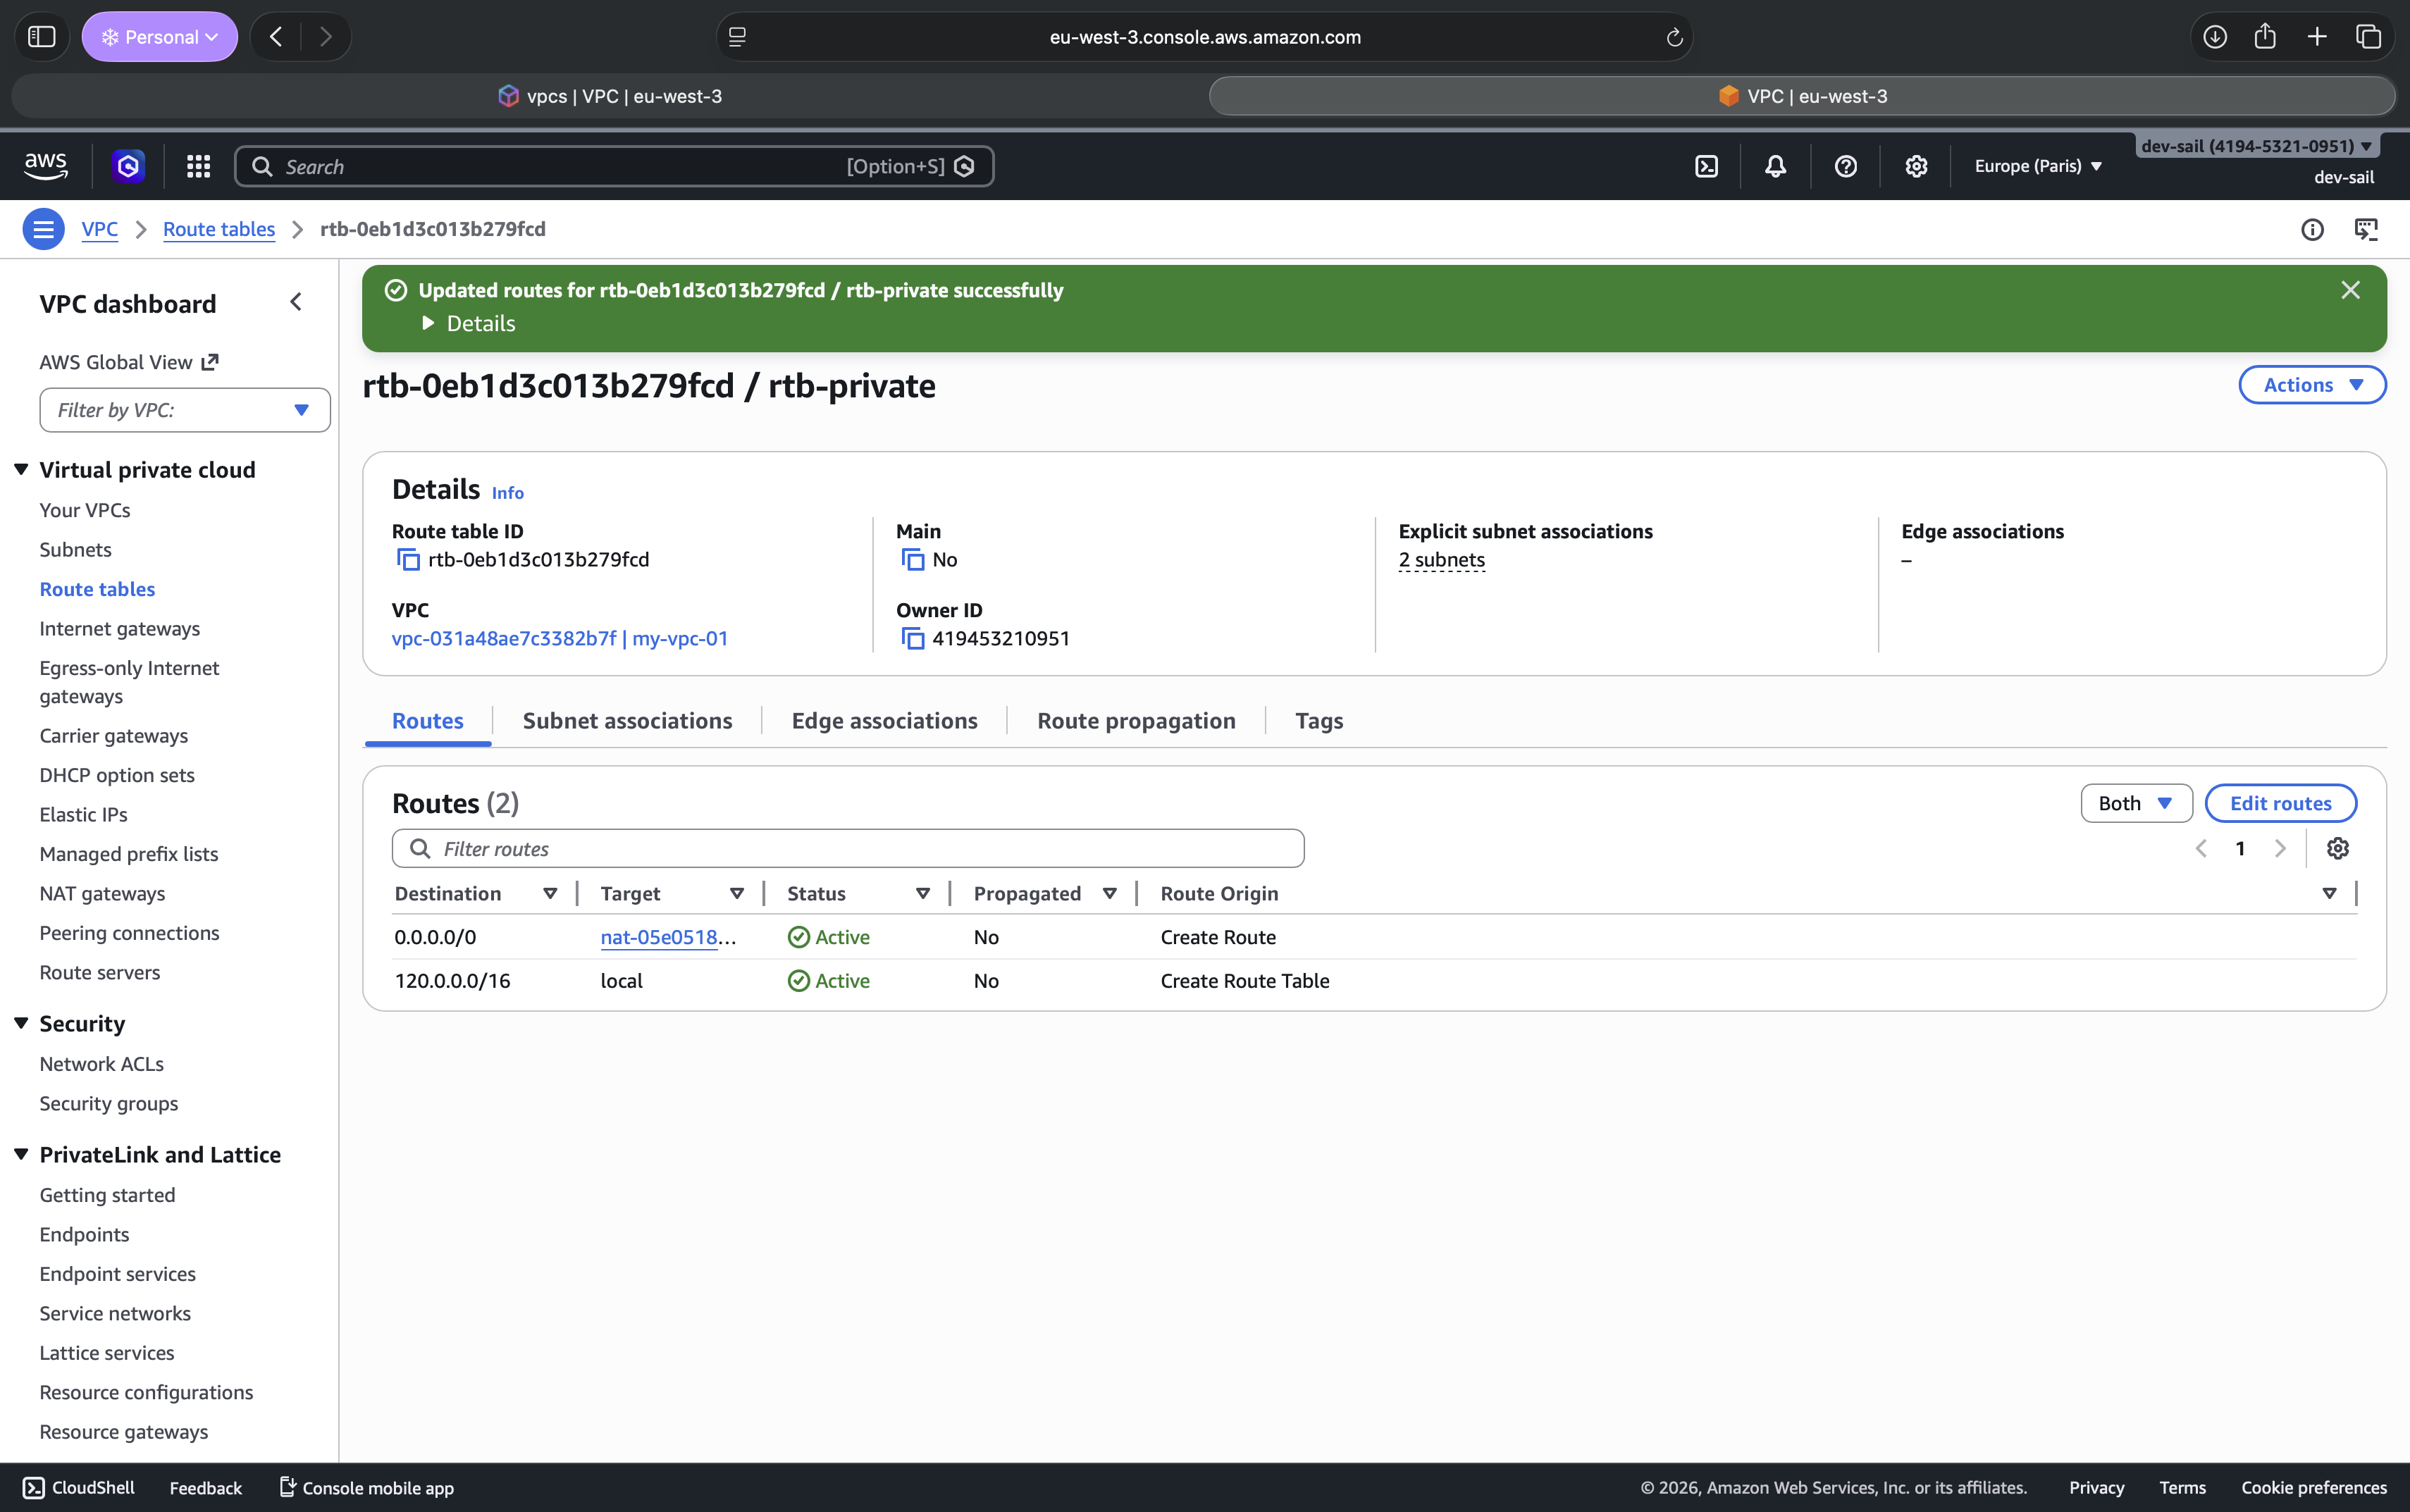
\includegraphics[width=0.75\textwidth]{figures/lab_3/private_route_table_with_nat_gateway.png}
\caption{Private route table with NAT Gateway}
\end{figure}

\end{document}
